\chapter{Konstrukce}
\label{4-algoritmus}

\section{Ovládání ESC (regulátorů otáček)}
Regulátor se ovládá přes různé komunikační protokoly. Komunikační protokoly jsou buď analogové nebo digitální. Mezi analogové protokoly patří standartní PWM signál, OneShot125, OneShot42 a MultiShot, mezi digitální patří  DSHOT300, DSHOT600 a DSHOT1200.\\
Standartní PWM signál není klasický PWM signál, kterým se například reguluje výkon žárovky. Standartní PWM signál definuje nulový výkon motoru pro pulz o délce 1ms a maximální výkon o délce 2ms. Teoretická frekvence je 500Hz, lze tedy měnit rychlost motorů 500krát za vteřinu.\\
Ostatní protokoly jsou sice rychlejší, ale nemá smysl je implementovat na platformu Arduino z důvodů malého výkonu platformy.\\ 

\begin{tabbing}
	Protokol ~~~~~~~~~ \= frekvence ~~~~~~~~~ \= min pulz us ~~~~~~ \= max pulz us
	\= 34 \kill
	\bfseries Protokol \>
	\bfseries Frekvece   \>
	\bfseries min pulz  \>
	\bfseries max pulz \\
	Standart PWM\> 500 Hz \> 1000µs  \> 2000µs  \\
	OneShot125\> 4 kHz \>  125µs \> 250µs   \\
	OneShot42\> 12 kHz \> 42µs \> 84µs \\
	MultiShot\> 40 kHz \> 12.5µs \> 25µs \\
\end{tabbing}

\begin{tabbing}
	Protokol ~~~~~~~~~ \= rychlost komunikace
	\= 34 \kill
		\bfseries Protokol \>
	\bfseries Rychlost komunikace   \\
	DSHOT150\> 150 000 bps \\
	DSHOT300\> 300 000 bps \\
	DSHOT600\> 600 000 bps  \\
	DSHOT1200\> 1200 000 bps \\
\end{tabbing}

\textbf{PWM}\\
PWM modulace je určená pro přenos analogového signálu pomocí dvou hodnot (Low a High), přenos probíhá na digitálních pinech. Přenášená hodnota je zaimplementována do poměru High/Low. Poměru se nazývá střída a nabývá hodnot 0-100 procent. Hodnoty Low a High se zapisují v cyklu. Pro příjem signálu je důležité znát frekvenci cyklu, aby mohlo dojít k dekódování a určení zaslané hodnoty.


%http://1oomzzme3s617r8yzr8qutjk-wpengine.netdna-ssl.com/wp-content/uploads/2017/04/Fig-1-pwm.gif
%pwm
\begin{figure}[h]
	\centering
	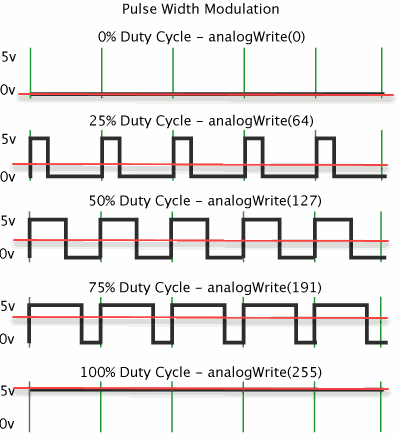
\includegraphics[width=10cm]{pictures/pwm.png}
	\caption{Ukázka PWM}
\end{figure}


\section{Kalibrace regulátorů otáček}
%https://www.youtube.com/watch?v=61bjFxJyOLU&t=52s
%blheli
Kalibrace regulátorů je nutná pro definování komunikačního protokolu a různých funkcí.\\
Pro kalibraci je potřeba kalibrovaný regulátor, propojovací dráty a Arduino Nano. V programu BLHeliSuite lze kalibrovat i s jinou platformu Arduino, bohužel kalibrace se podařila pouze s deskou typu Nano.\\
Zapojení regulátoru se proveve přes schéma na obrázku 5.2.\\
Po zapojení komponent a nastavení šablony se vybere sériový port pro komunikaci mezi počítačem a Arduinem. Přes tlačítko Read Setup se načte tovární nastavení regulátoru.\\
Nastaví se PPM Min Throttle hodnota na 1000, PPM Max Throttle na 2000 a PPM Center Throttle na 1500. Zapíše se hodnota do regulátoru. Tím se zkalibrovaly vstupní hodnoty pulzu do intervalu <1000;2000>. \\
Při každém zapnutí motoru je potřeba jiná kalibrace a to posláním příkazu s hodnotou Min Throttle a následně Max Throttle.



\begin{figure}[h]
	\centering
	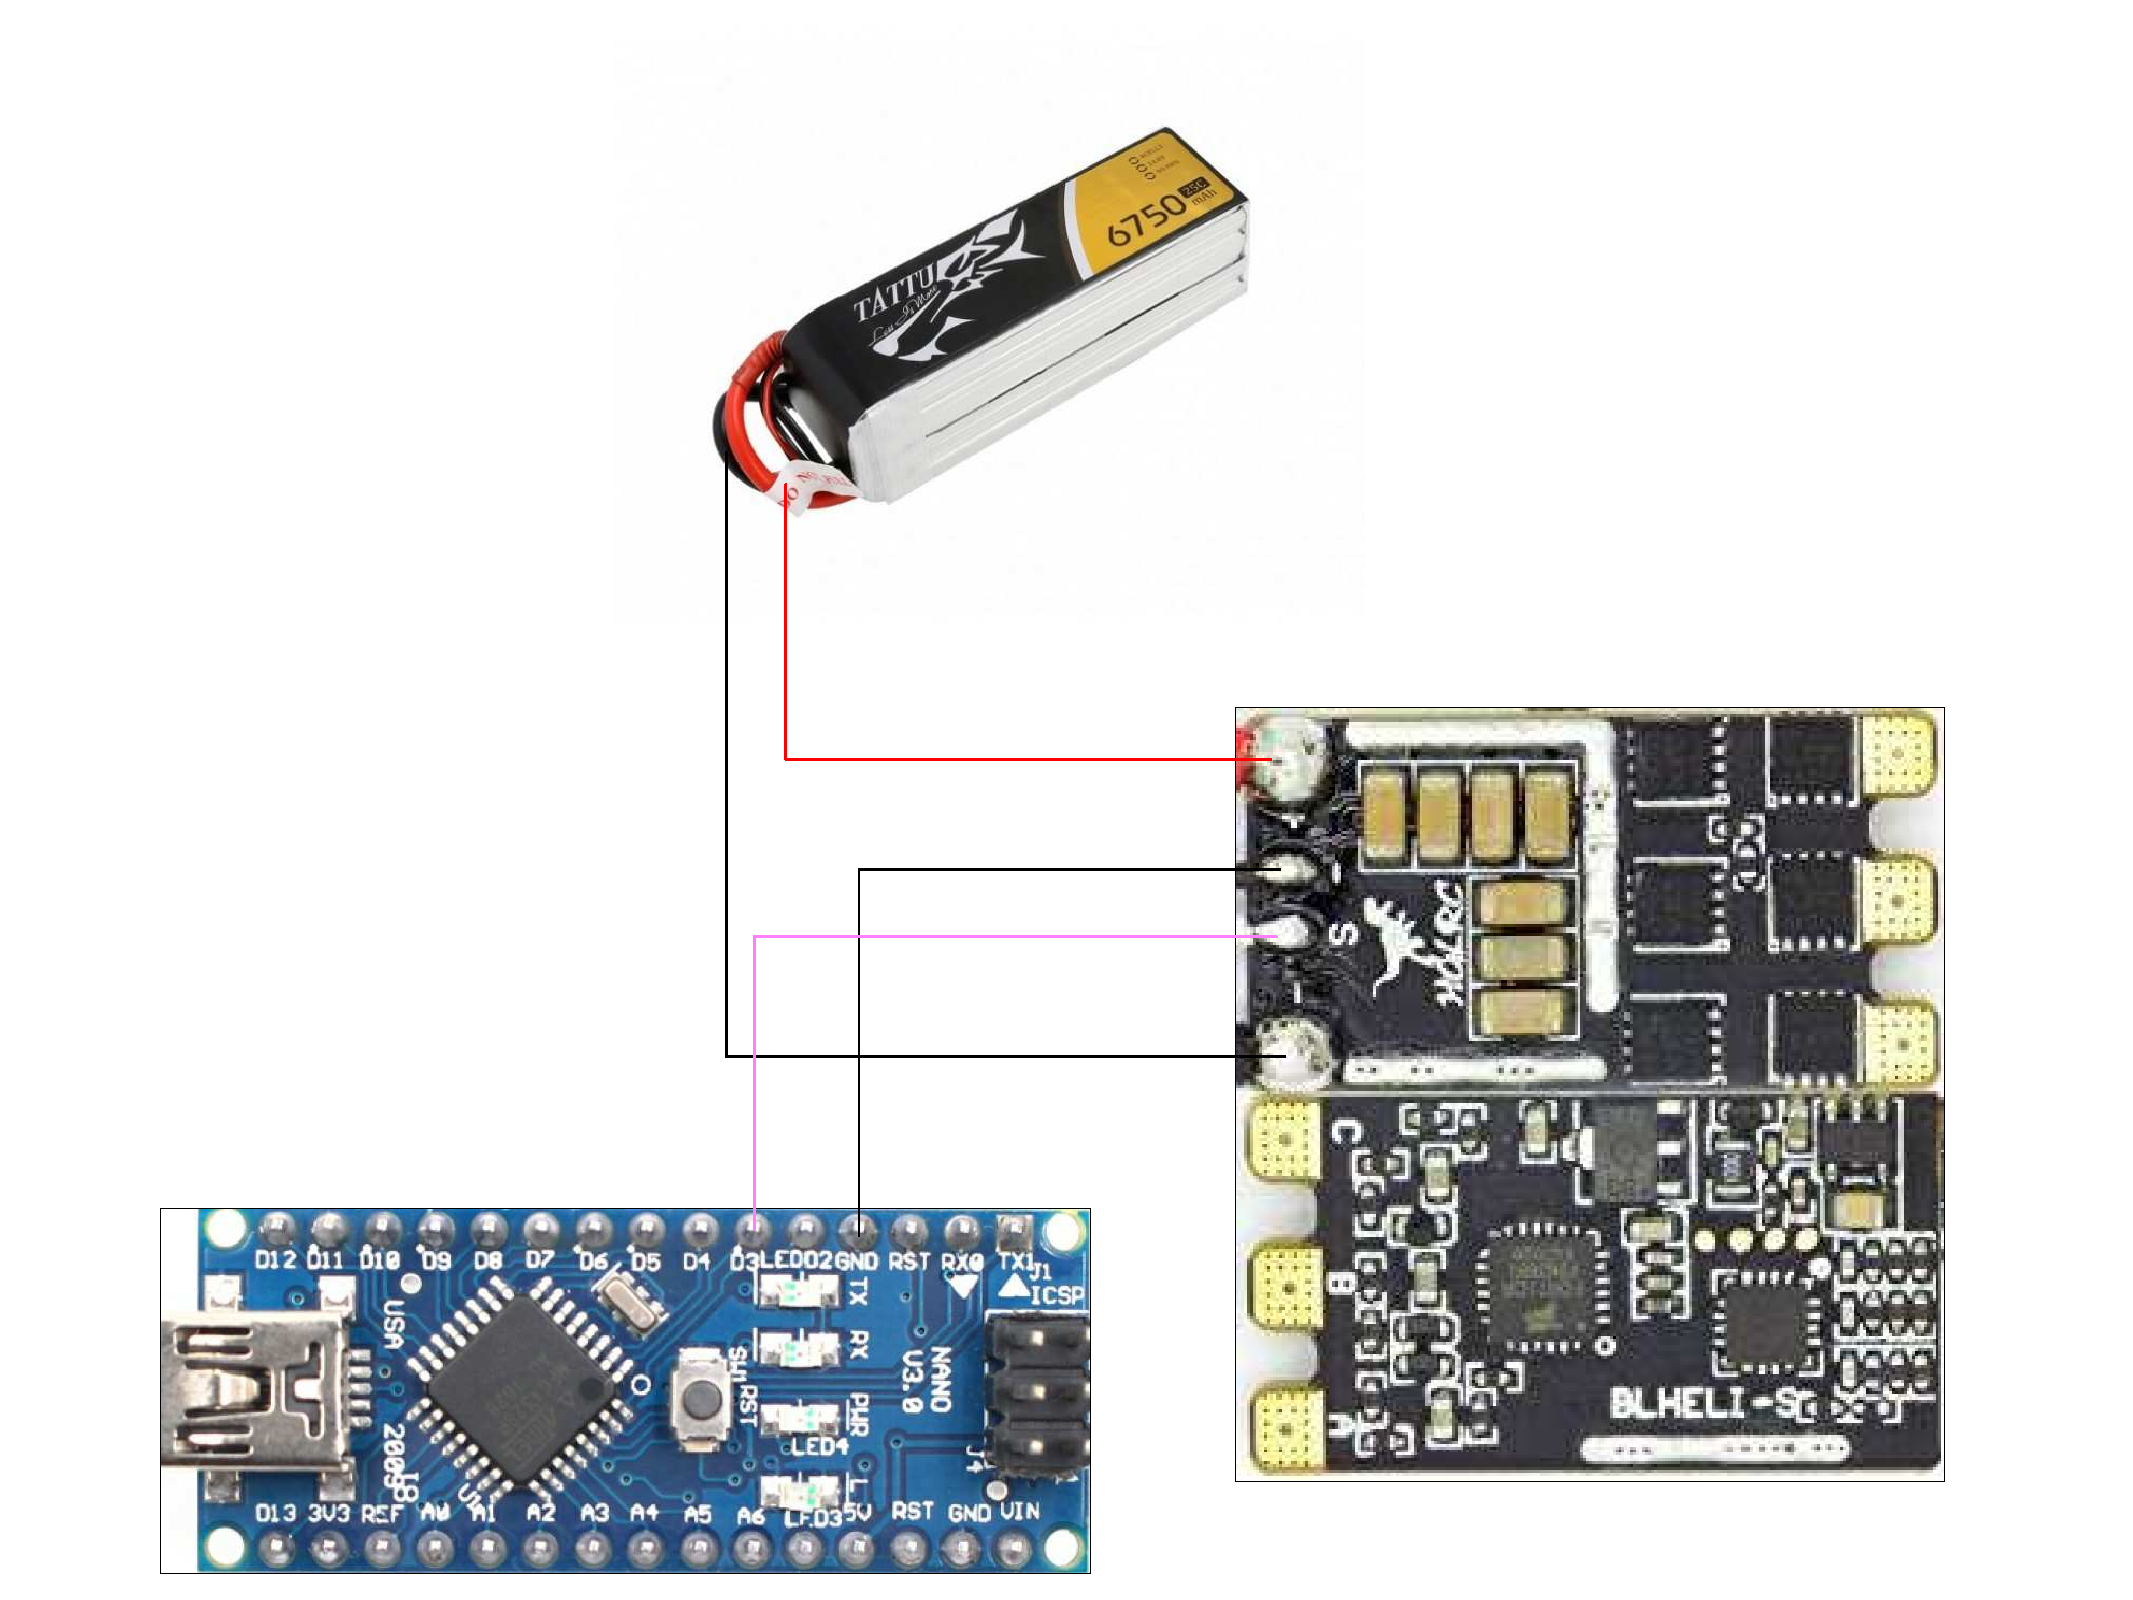
\includegraphics[width=12cm]{pictures/esc_calib.pdf}
	\caption{Schéma zapojení pro kalibraci regulátoru otáček}
\end{figure}

\begin{figure}[h]
	\centering
	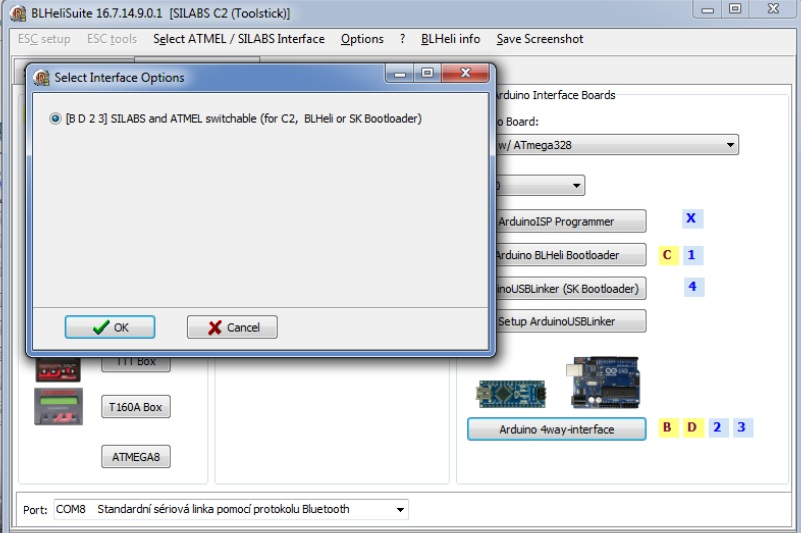
\includegraphics[width=12cm]{pictures/esc_calib1.jpg}
	\caption{Schéma zapojení pro kalibraci regulátoru otáček}
\end{figure}

\begin{figure}[h]
	\centering
	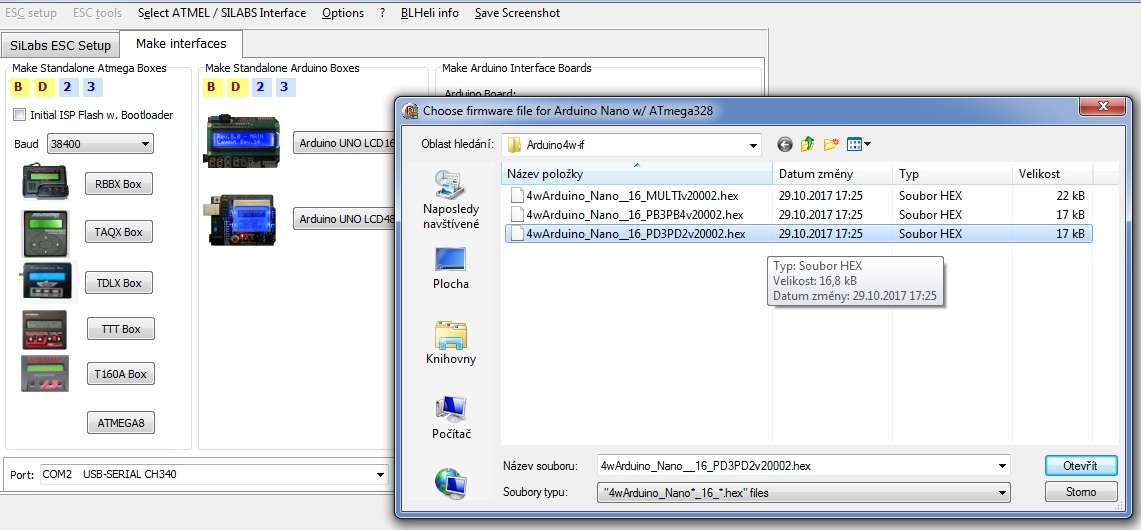
\includegraphics[width=12cm]{pictures/esc_calib2.jpg}
	\caption{Schéma zapojení pro kalibraci regulátoru otáček}
\end{figure}

\begin{figure}[h]
	\centering
	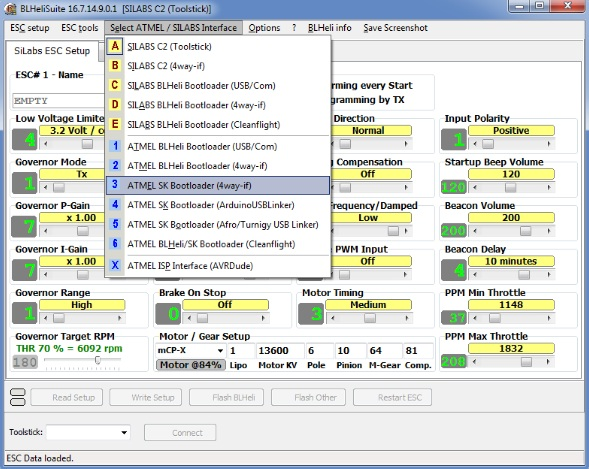
\includegraphics[width=12cm]{pictures/esc_calib3.jpg}
	\caption{Schéma zapojení pro kalibraci regulátoru otáček}
\end{figure}

\section{Filtrace dat IMU}

%\begin{eqnarray*} 
%	pitchAcc & = & atan2( yAcc, sqrt{xAcc$^2$+ zAcc$^2$}) * (180/PI) \\
%
%\end{eqnarray*} 
%
%\begin{eqnarray*} 
%	rollAcc & = & 168.75A\\
%%		accY = atan2(-1 * (aX) , sqrt(pow(aY, 2) + pow(aZ, 2)))  * (180 / M_PI);
%\end{eqnarray*} 

%  gyroX = pitch + gX  * elapsedTime / 10e6;
%gyroY = roll + gY * elapsedTime / 10e6;

Surová data ze všech tří senzorů nejsou použitelná pro výpočet úhlů náklonu, obsahují nepřesnosti a šum, proto je potřebná filtrace.\\

%https://aip.scitation.org/doi/pdf/10.1063/1.5018520

\subsection{Komplementární filtr}
Komplementární filtr je nejjednodušší z uvedených filtrů. Využívá data z akcelerometru a gyroskopu. \\
Z dlouhodobého hlediska data z gyroskopu konvergují. Z krátkodobého hlediska jsou přesná, proto pro další použití je potřeba použít High Pass filtr.\\
Opakem toho jsou data z akcelerometru, data jsou ovlivňována malými silami, které ruší výsledné zrychlení. Z dlouhodobého hlediska jsou data z akcelerometru přesná, proto je potřeba použít Low Pass filtr.\\
Kombinací High Pass filtru a Low Pass filtr vzniká komplementární filtr, který je pro použití při ovládání dronu dostačující.\\


\subsection{Kalmanův filtr}
Kalmanův filtr je dynamický filtr, který pracuje s predikcí. Pro výpočet je potřeba stanovit model systému, u kterého bude filtr predikovat stavy. Pokud v oblasti predikovaného stavu najdeme skutečný stav, provede se korekce skutečného stavu a oblast predikovaného stavu bude menší/přesnější. Nenalezne-li se v oblasti predikovaného stavu skutečný stav, oblast se zvětší/zhorší se přesnost.\\
Bohužel Kalmanův filtr nemohl být použít z důvodu malé výpočetní síly platformy Arduino.

\subsection{Mahonyho filtr}
Mahonyho filtr využívá Quaternions, což je čtyř dimensionální numerický systém využívaný pro popis rotace objektu v počítačové grafice a robotice. Filtr používá data z gyroskopu, akcelerometru a magnetometru, přičemž z nich počítá úhly pitch, roll a yaw. Při výpočtu použita knihovna MahonyAHRS.\\
%https://github.com/PaulStoffregen/MahonyAHRS
mahony
%https://www.youtube.com/watch?v=zjMuIxRvygQ

\section{PID regulátor pro synchornizaci motorů} 
Proportional Integral Derivative
PID regulátor slouží k regulaci požadovaného stavu v nejkratší době a to za pomocí zvyšování a snižování vlivu, který napomáhá dostat se do požadovaného stavu.\\
Názorný příklad:
Požadujeme, aby dron držel stabilní polohu, chceme, aby proměnné pitch a roll z IMU byly nulové. Kdybychom měli ideální dron s přesným vyvážením hmotnosti a se stejně fungujícími motory, bylo by to snadné. Pouze by stačilo zapsat stejnou hodnotu na všech motorech a dron by bez problémů vzlétnul. Bohužel ideální dron nemáme, proto motory se musí být ovládany individuálně.\\
PID regulátor reaguje na tzv. errory (odchylky od požadovaného stavu) a následně přes koeficienty kp, ki a kd spočte hodnoty pro ovládání motorů.
PID regulátor má tři složky: proporcionální (kp), integrační (ki) a derivační (kd).\\
Proporcionální složka ovlivňuje ovládání motorů lineárně. Pokud je odchylka veliká zvýší se rychlost na motorech, pokud je odchylka nulová, motory se plně zastaví a spustí se až když je odchylka není nulová.\\
Integrační složka ovlivňuje ovládání motorů v závislosti na předchozím stavu. Pokud je odchylka velká, integrační složka se zvětšuje do doby dokud nedosáhne požadovaného stavu, potom se integrační složka zmenšuje a mění svoje znaménko.\\
Derivační složka reaguje na změnu rychlosti odchylky. Čím rychleji se bude odchylka měnit, tím větší bude vliv derivační složky. Derivační složka reaguje proti P a I složce.\\
Pro autonomní řízení dronu bude celkem potřeba šest PID regulátorů viz obr..\\
\newpage
\begin{figure}[h]
	\centering
	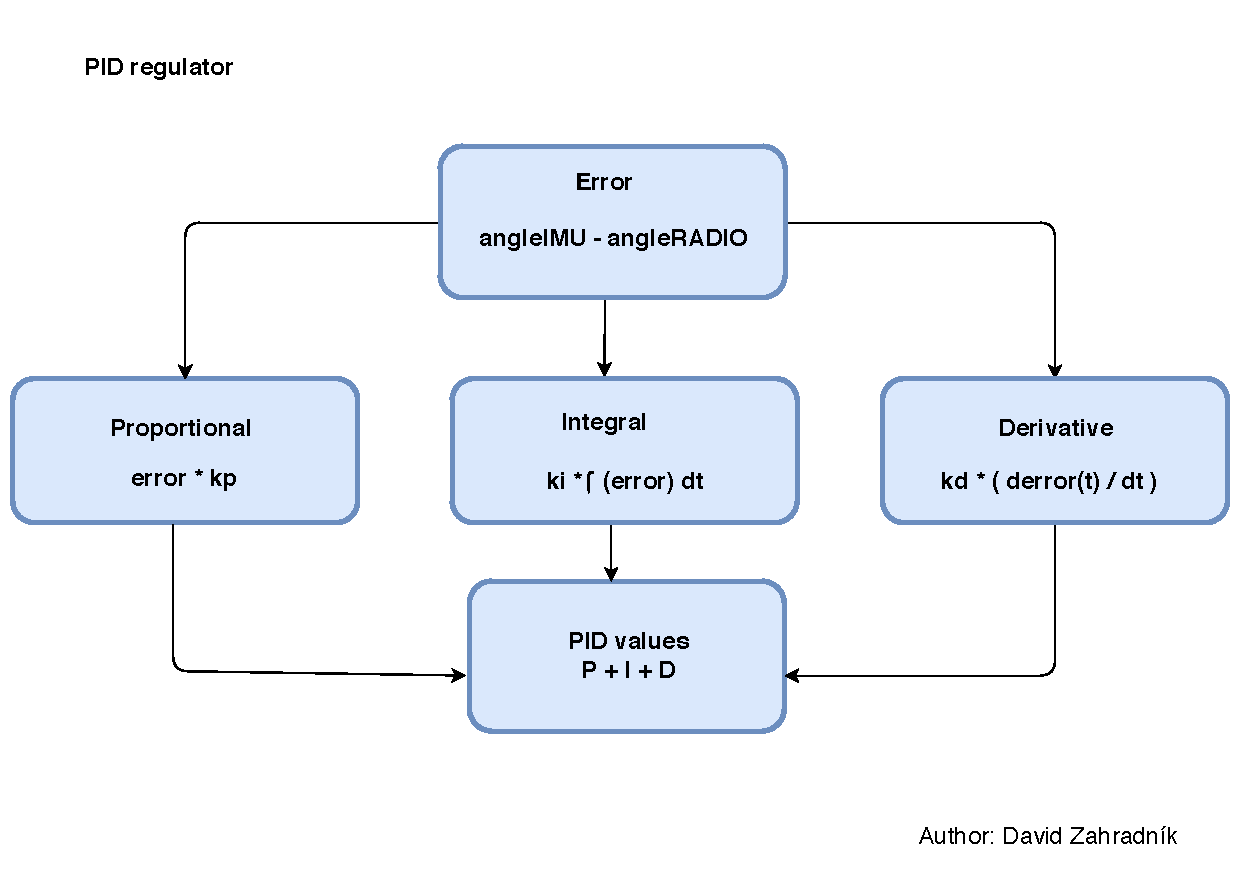
\includegraphics[width=15cm]{pictures/PIDDiagram.pdf}
	\caption{Schéma PID regulátoru}
\end{figure}

\begin{figure}[h]
	\centering
	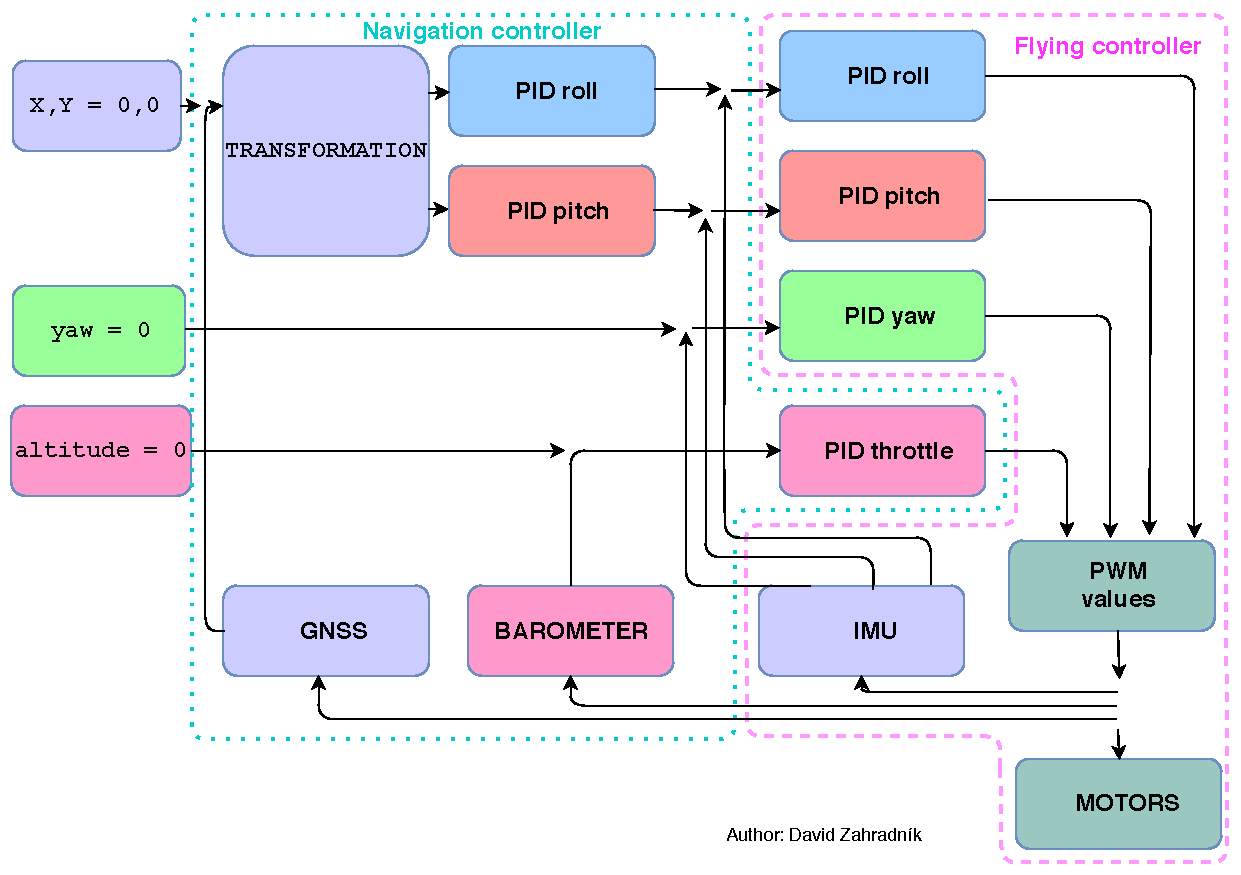
\includegraphics[width=15cm]{pictures/PIDsDiagram.pdf}
	\caption{Schéma všech PID regulátorů při stavbě dronu}
\end{figure}


\begin{figure}[h]
	\centering
	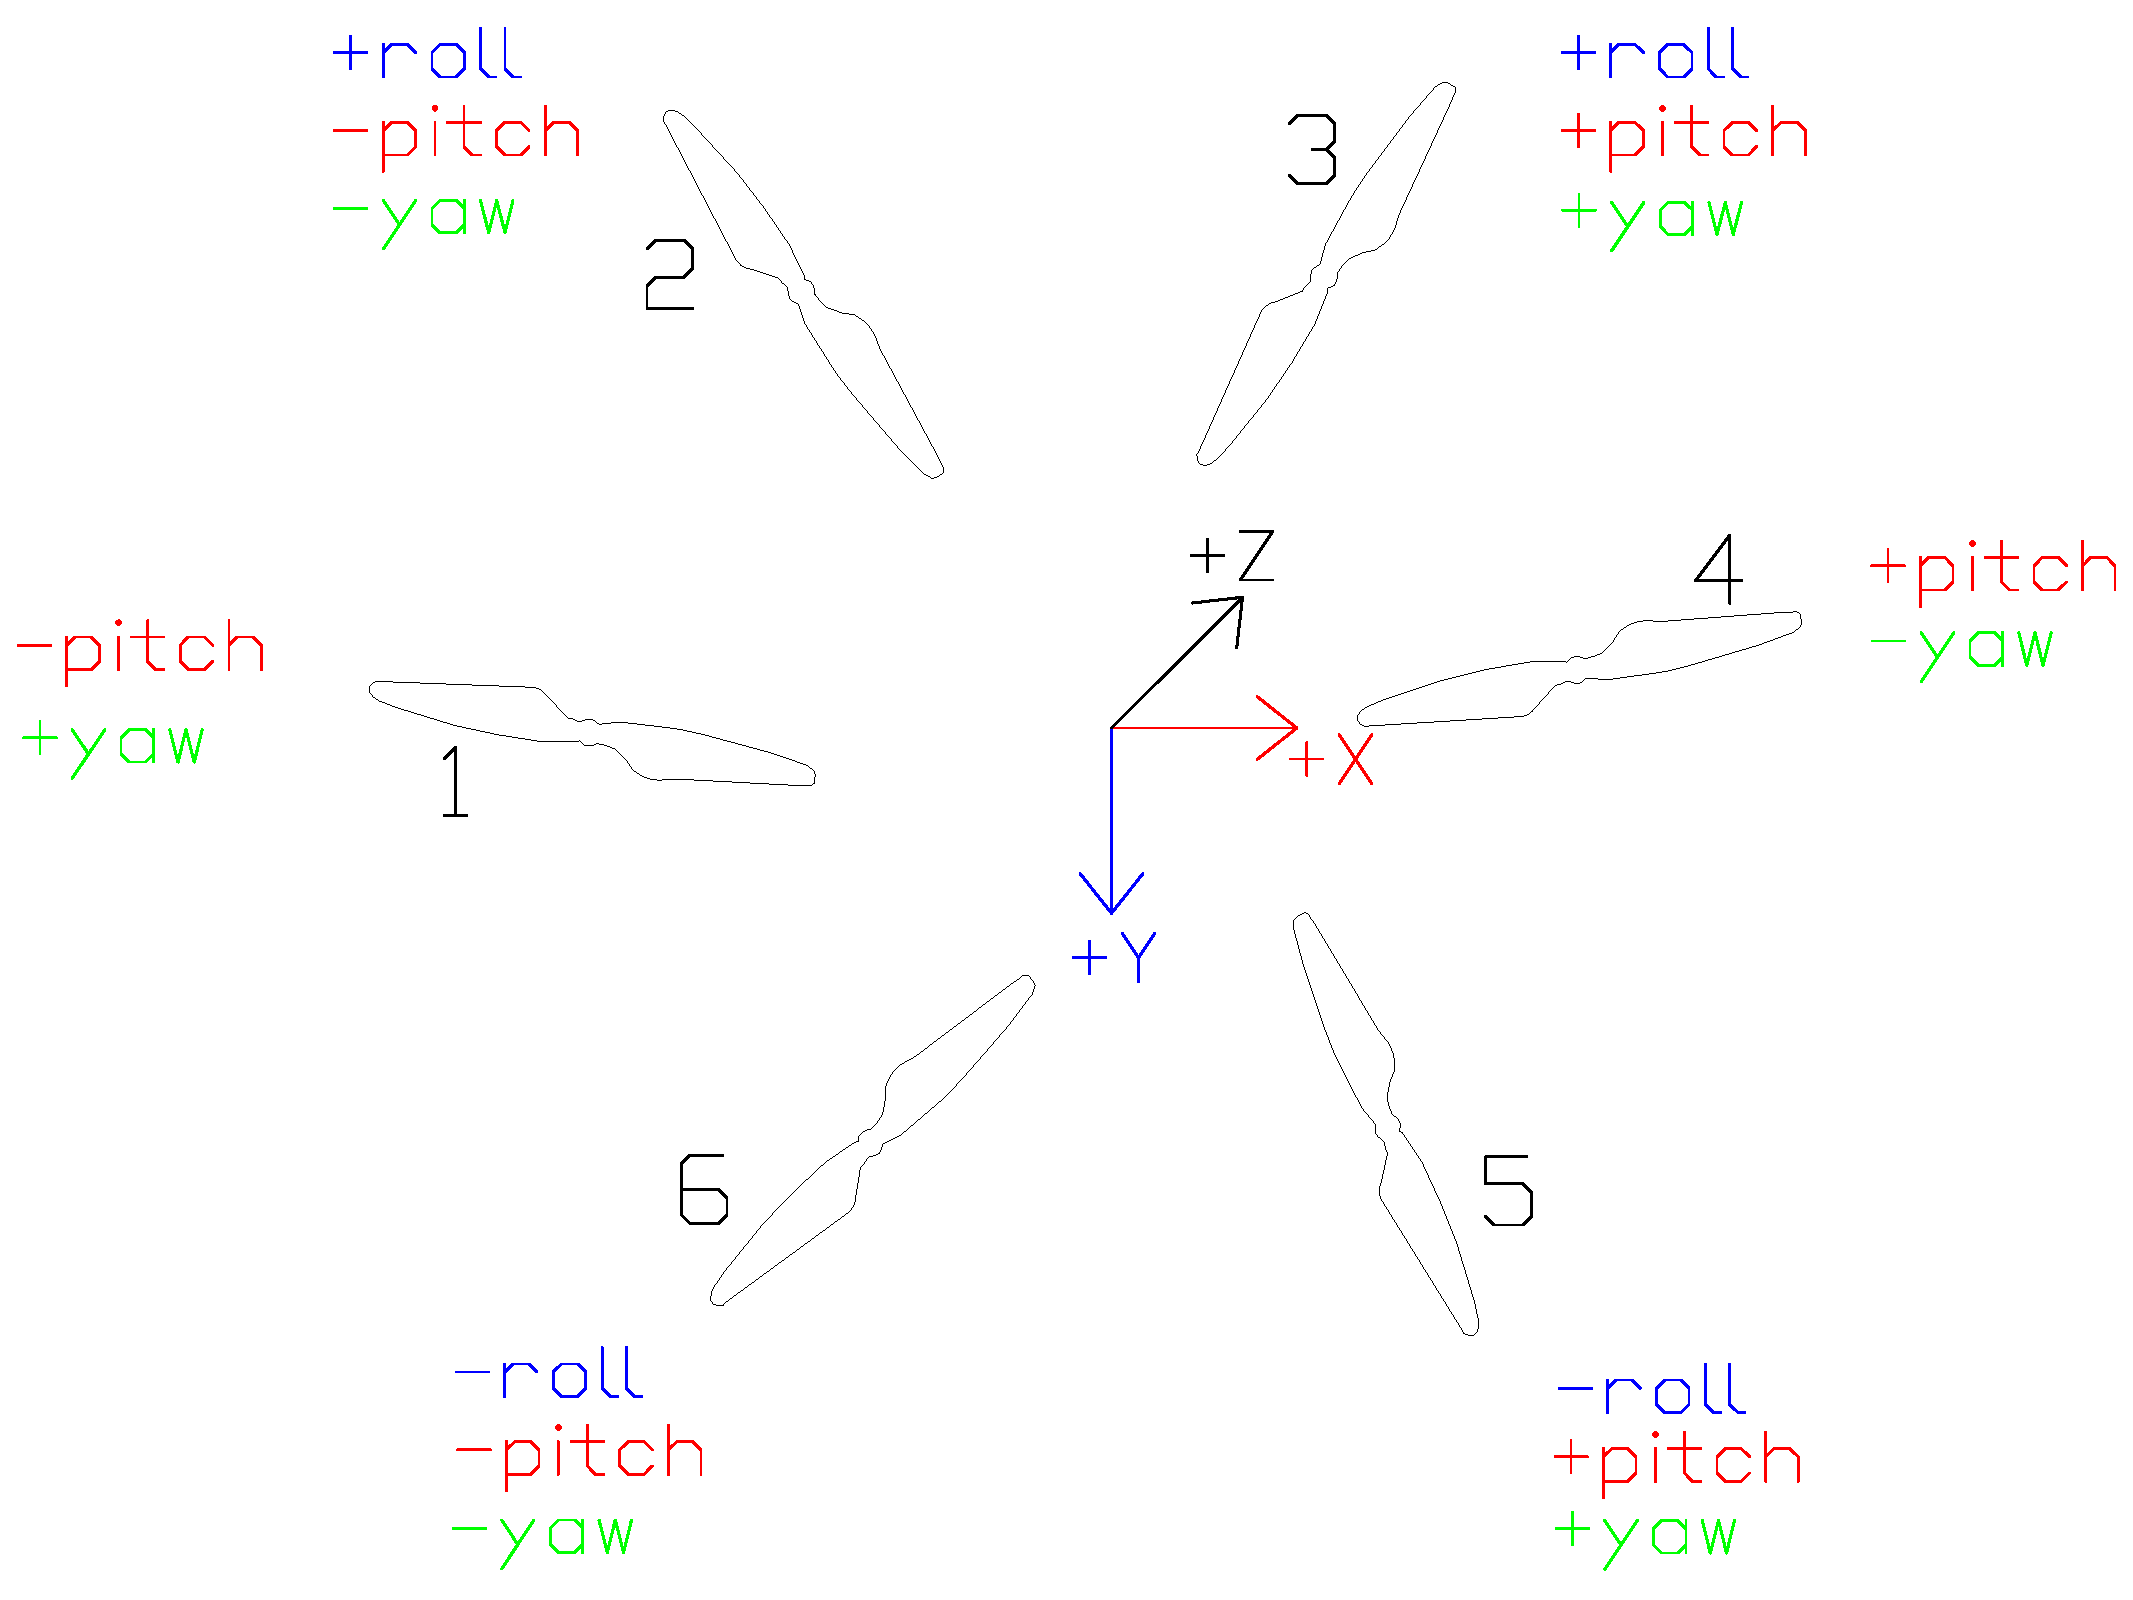
\includegraphics[width=12cm]{pictures/pid.pdf}
	\caption{Schéma ovládání vrtulí podle úhlu náklonu}
\end{figure}
%https://valter.byl.cz/plynula-regulace-pid
pid
%http://www.controlengcesko.com/hlavni-menu/artykuly/artykul/article/derivacni-slozka-v-regulaci-pid/

\section{Komunikační protokol}
Pro propojení dronu a smartphonu je použita bluetooth a radiová komunikace. Komunikace je realizována přes sériové rozhraní UART. UART lze implementovat pouze mezi dvěma zařízeními, komunikace je oboustranná na rozdíl od I2C a SPI. Pro realizaci komunikace je nutné nastavit stejnou rychlost komunikace (bps).\\
Pro použití rozhraní UART byl vytvořen komunikační protokol pro ovládání dronu. Začátek zprávy je definován znakem < a konec zprávy >. Hodnoty potřebné pro ovládání jsou určeny prvním bytem (znakem) a hodnota následující dvěma byty. Hodnota dána čísly 0-99 se interpoluje do rozsahu uvedeného v tabulce.\\

\begin{tabbing}
	Zprava ~~~ \= uhel ~~~~~~~~~~~~~~ \= od ~~~~~~~~~ \= do ~~~~~~
	\= 34 \kill
	\bfseries Znak \>
	\bfseries Typ hodnoty \>
	\bfseries Od \>
	\bfseries Do \\
	T\> Throttle \> 1000 µS \> 1700 µS \\
	P\> Pitch \>  -25$^\circ$ \> +25$^\circ$   \\
	R\> Roll \> -25$^\circ$ \> +25$^\circ$ \\
	Y\> Yaw \> 0$^\circ$ \> 360$^\circ$ \\
	C\> kalibrace \> null \> null \\
	H\> návrat \> null \> null \\
	F\> zem. šířka \> null \> null \\
	L\> zem. délka \> null \> null \\
	D\> stupně \> 48$^\circ$ (12$^\circ$)\> 51$^\circ$(19$^\circ$) \\
	M\> minuty \> 0´ \> 60´ \\
	S\> sekundy \> 0´´ \> 60´´ \\
	
\end{tabbing}

\section{Radiová komunikace XBEE}
Před zahájením komunikace mezi radiovými moduly je nutné provést jejich konfigurace. Ke konfiguraci slouží program XCTU (Linux, Windows), od výrobců modulů XBEE. Pro propojení počítače a modulu lze použít shield (nadstavbové zařízení k mikrokontrolérům) od firmy Digi, nebo je možné využít platformu Arduino a XBEE shield.\\
K propojení radiového modulu a počítače s pomocí platformy Arduino je potřeba udělat pár kroků. V první řadě se do platformy nahraje jednoduchý kód, který bude mít za úkol číst data z počítače a posílat je radiovému modulu. V kód je třeba definovat, na kterých pinech bude prováděna komunikace s radiovým modulem. Druhý krok je nastavení pinů pro komunikaci s radiovým modulem na shieldu. V posledním kroku se složí všechno dohromady.\\
Nejdůležitějšími nastaveními radiových modulů jsou definování funkce, rychlost komunikace (bps) a ID sítě. V síti radiových modulů je potřeba jeden koordinátor, na počtu routerů a koncových zařízení nezáleží. Koordinátor obstarává inicializaci sítě a umožnuje dalším modulů se připojit do sítě. Router funguje jako prostředník při přenosu dat. Koncové zařízení slouží buď k příjmu a odesílání zpráv. Rychlost komunikace je dána přenosem bitů za sekundu (bps), rychlost komunikace musí být totožná na všech zařízeních v síti. ID sítě slouží k uzavření komunikace jenom mezi určitými radiovými moduly.\\
%https://www.tunnelsup.com/xbee-guide/
%xbeetut

\begin{figure}[h]
	\centering
	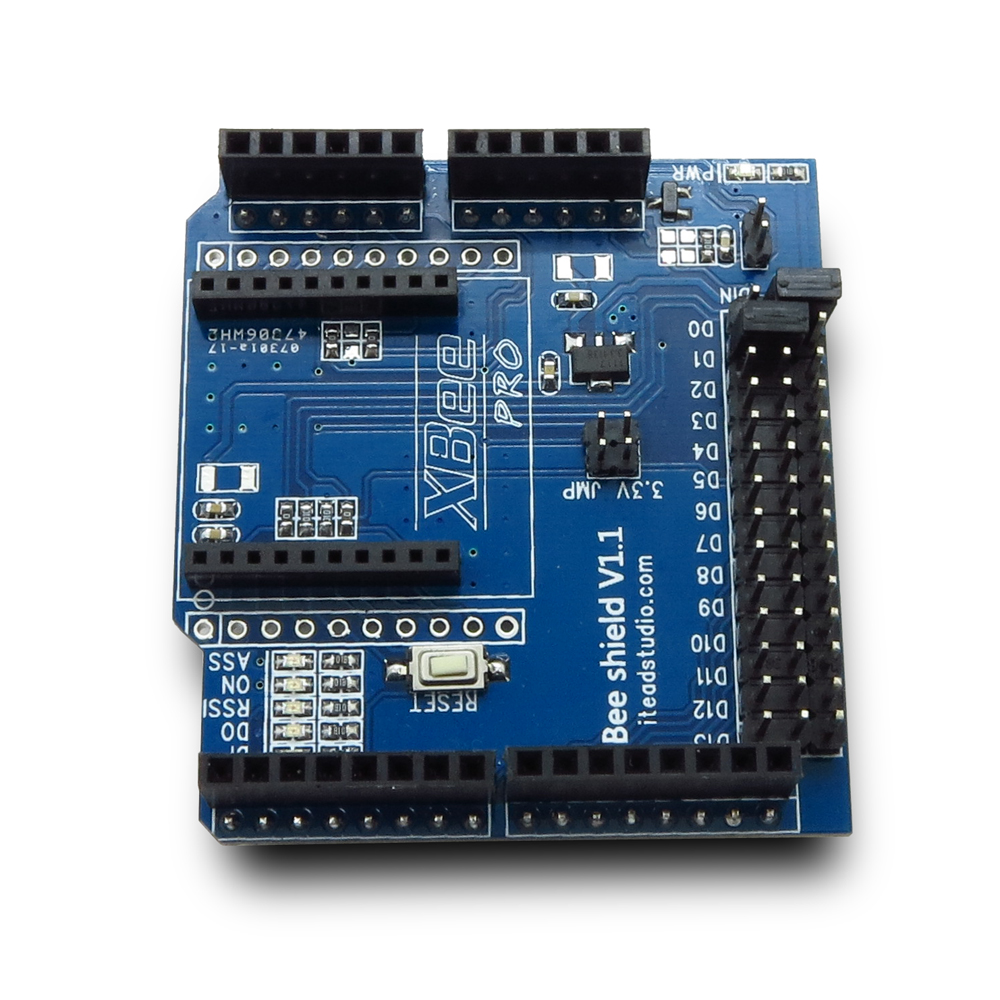
\includegraphics[width=8cm]{pictures/xbeeshield.jpg}
	\caption{XBEE shield}
\end{figure}


\section{Letový kontrolér} 
Vstup: IMU, Navigační kontrolér\\
Výstup: ESC\\

Letový kontrolér slouží k synchronizaci a ovládání motorů dronu. Letový kontrolér zpracovává měření z IMU a porovnává jej s daty z navigačního kontroléru (pitch, roll a yaw). Pokud úhly náklonů nejsou totožné, kontrolér přes PID regulátor změní rychlost motorů tak, aby úhly ztotožnil.\\
Při spuštění letový kontrolér provede kalibraci regulátorů otáček zapsáním minimální a maximální hodnotu výkonu.\\
Po proběhnutí kalibrace regulátorů otáček, kontrolér čte data z IMU, probíhá filtrace pomocí komplementárního filtru a počítá úhly pitch, roll a yaw.\\
Z navigačního kontroléru jsou získávána data, která jsou následně separována a interpolována do požadovaných hodnot. Hodnoty se rozlišují prvním bytem, který definuje o jakou hodnotu se jedná. Další dva byte představují číslo od 0 do 99, které se vyinterpoluje na požadovaný rozsah.\\

\begin{tabbing}
	Zprava ~ \= uhel ~~~~~~~~~ \= od ~~~~~~~ \= do ~~~~
	\= 34 \kill
	\bfseries Byte \>
	\bfseries Zpráva \>
	\bfseries Od \>
	\bfseries Do \\
	T\> Throttle \> 1000 µS \> 1700 µS \\
	P\> Pitch \>  -25$^\circ$ \> +25$^\circ$   \\
	R\> Roll \> -25$^\circ$ \> +25$^\circ$ \\
	Y\> Yaw \> 0$^\circ$ \> 360$^\circ$ \\
\end{tabbing}

Hodnota výkonu motoru/throttle se vyinterpoluju pouze do 1700 µS, protože ke konstantnímu výkonu se ještě připočítávají údaje z PID regulátoru. Rozsah dat z PID regulátoru je <-300;300>, pokud by se zapsal konstaní výkon větší než 1700 µS, PID regulátor by byl omezen.\\
Hodnota náklonů pitch a roll  může být nejvýše 25 stupňů, kdyby byla hodnota větší hrozilo by převrácení dronu.\\
Z rozdílu úhlů z IMU a navigačního kontroléru se vypočtou odchylky. Podle odchylek se vyčíslí proporcionální, integrační a derivační složka PID regulátoru každého úhlu. Součet všech tři složek představuje změnu výkonu motoru pro jednotlivý úhel. Dle pohybových rovnic pro každý motor se vypočtou výkony motorů.

\begin{eqnarray*} 
	motor1 & = & throttle - pidPitch           + pidYaw\\
	motor2 & = & throttle - pidPitch + pidRoll - pidYaw\\
	motor3 & = & throttle + pidPitch + pidRoll + pidYaw\\
	motor4 & = & throttle + pidPitch           - pidYaw\\
	motor5 & = & throttle + pidPitch - pidRoll + pidYaw\\
	motor6 & = & throttle - pidPitch - pidRoll - pidYaw\\
\end{eqnarray*} 

\begin{figure}[h]
	\centering
	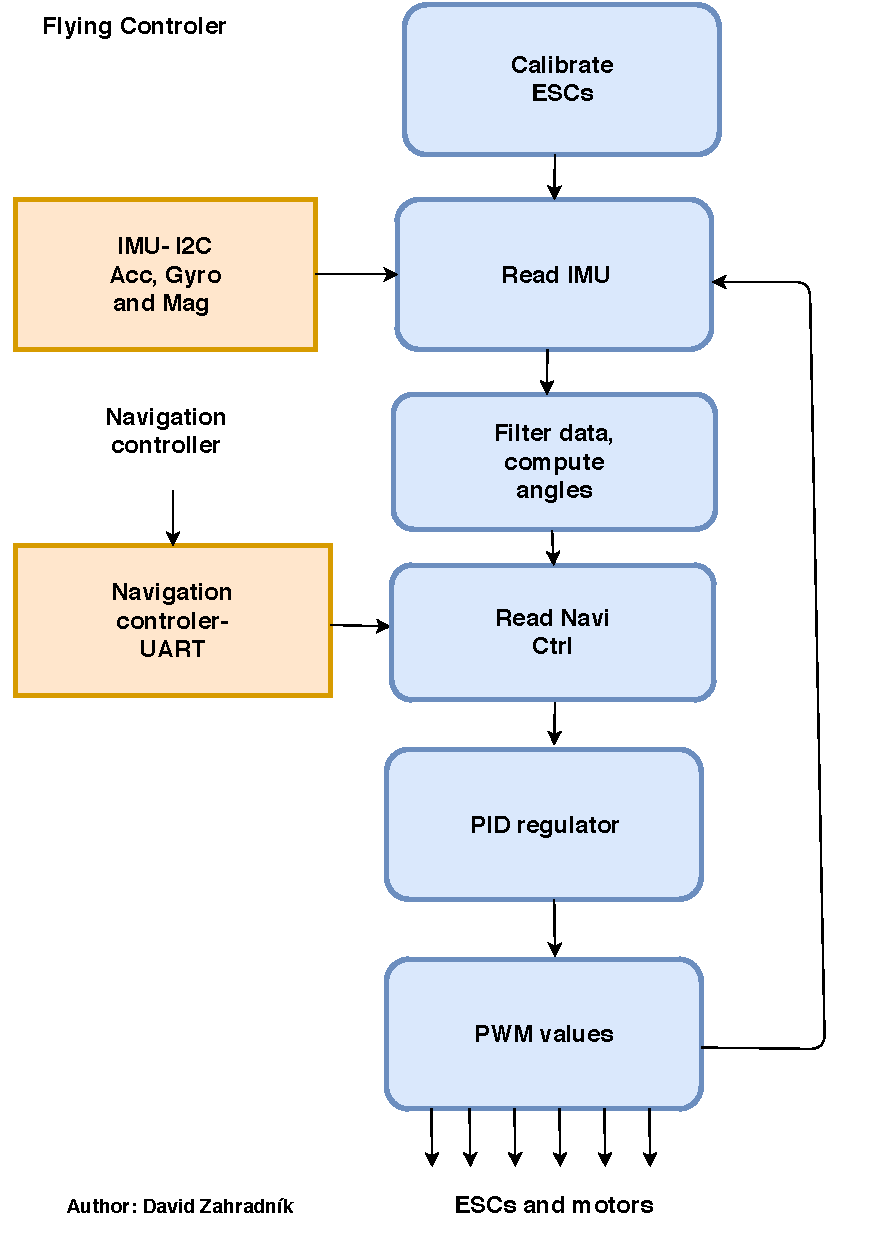
\includegraphics[width=12cm]{pictures/FlyingDiagram.pdf}
	\caption{Diagram algoritmu letového kontroléru}
\end{figure}


\begin{figure}[h]
	\centering
	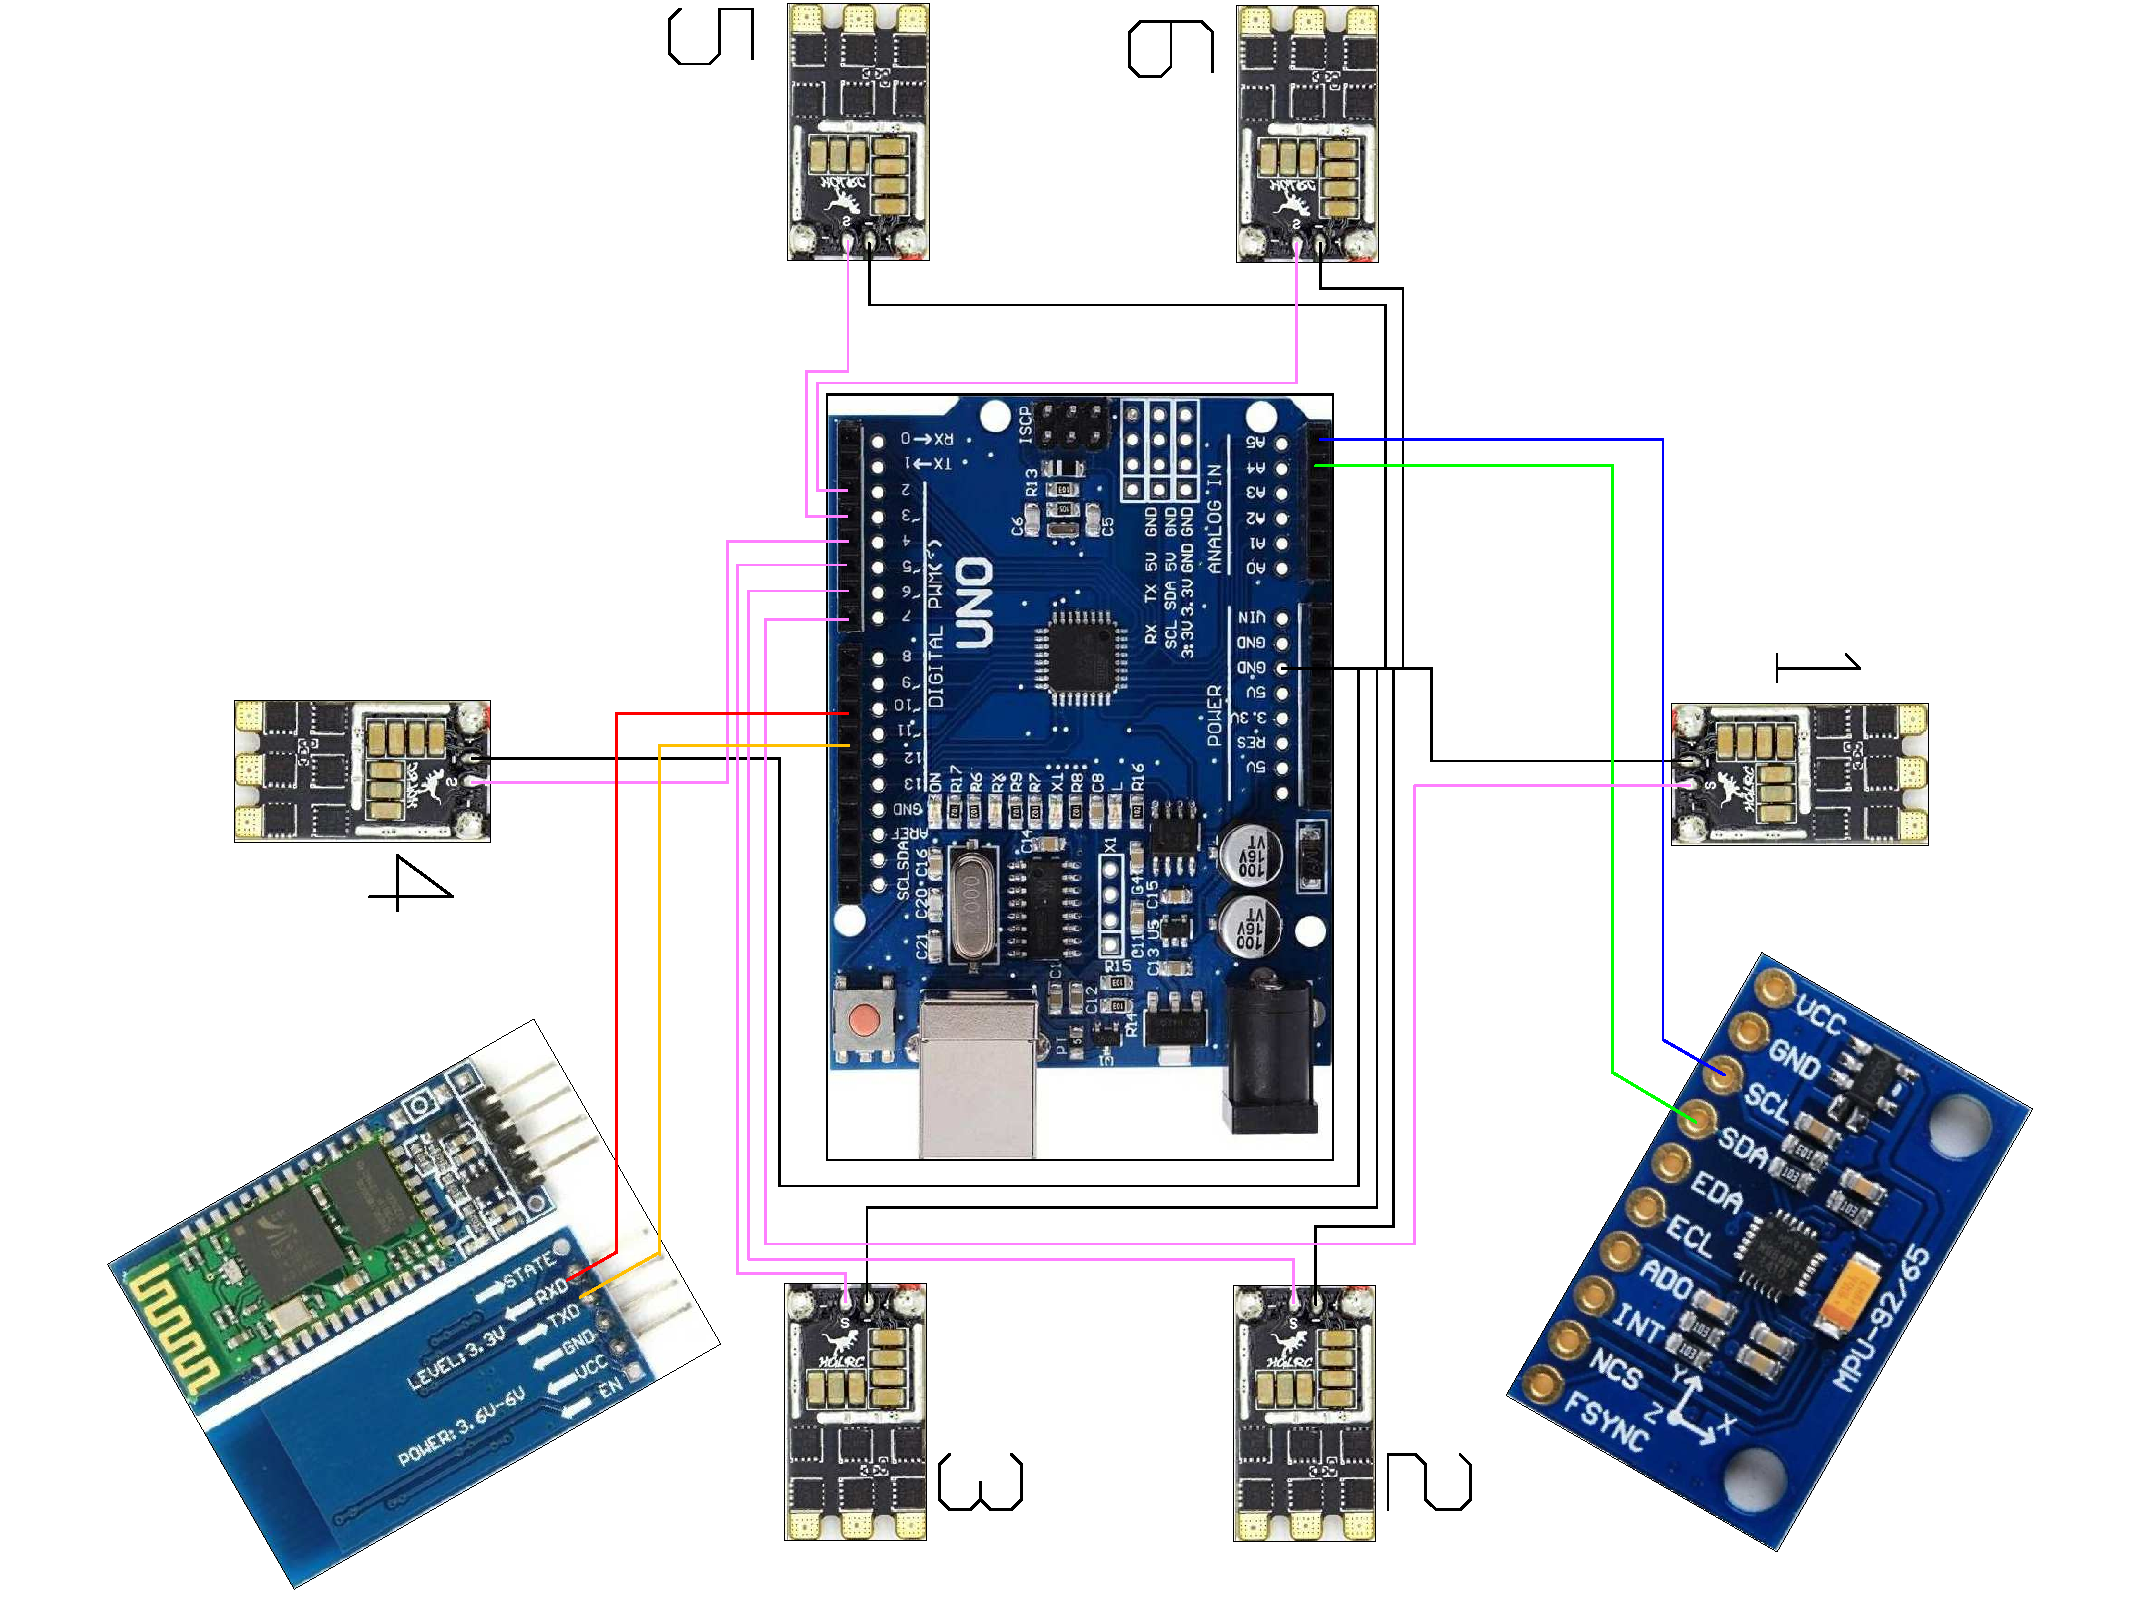
\includegraphics[width=12cm,angle=90]{pictures/flyctrl.pdf}
	\caption{Schéma zapojení letového kontroléru}
\end{figure}

\section{Překážkový kontrolér} 
Vstup: 7x laserový modul\\
Výstup: Navigační kontrolér\\

Překážkový kontrolér má za úkol zabránit kolizi dronu s cizím objektem. Laserové moduly jsou nasměrovány do směrů pohybu podle úhlů pitch, roll a jeden laser je nasměrován po svislici pro přistávání. Lasery jsou nastaveny na kontinuální měření vzdáleností. Pokud v blízkosti se nachází cizí objekt, kontrolér pošle zprávu o existují překážce navigačnímu kontroléru a její poloze.\\

\begin{figure}[h]
	\centering
	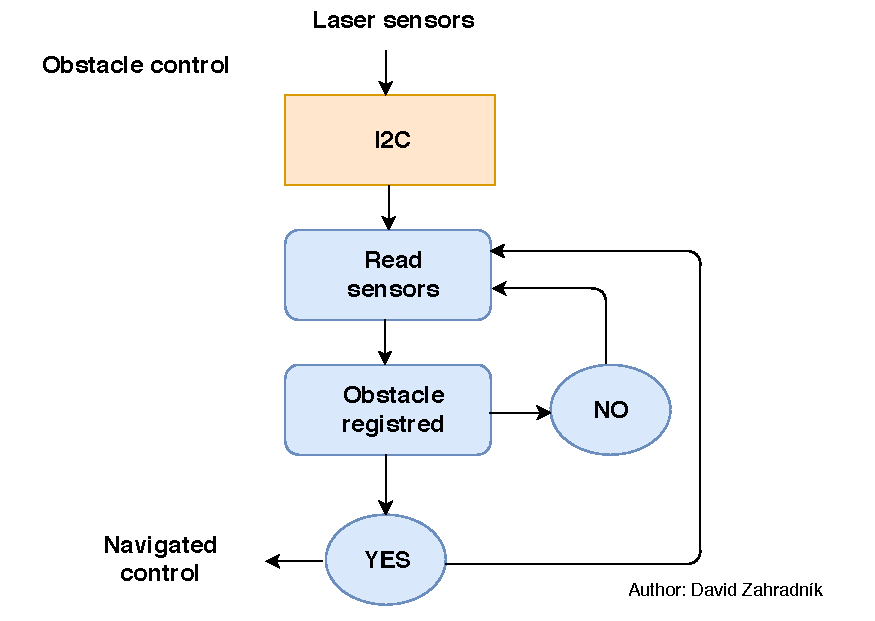
\includegraphics[width=12cm]{pictures/ObstacleDiagram.pdf}
	\caption{Diagram algoritmu překážkového kontroléru}
\end{figure}

\begin{figure}[h]
	\centering
	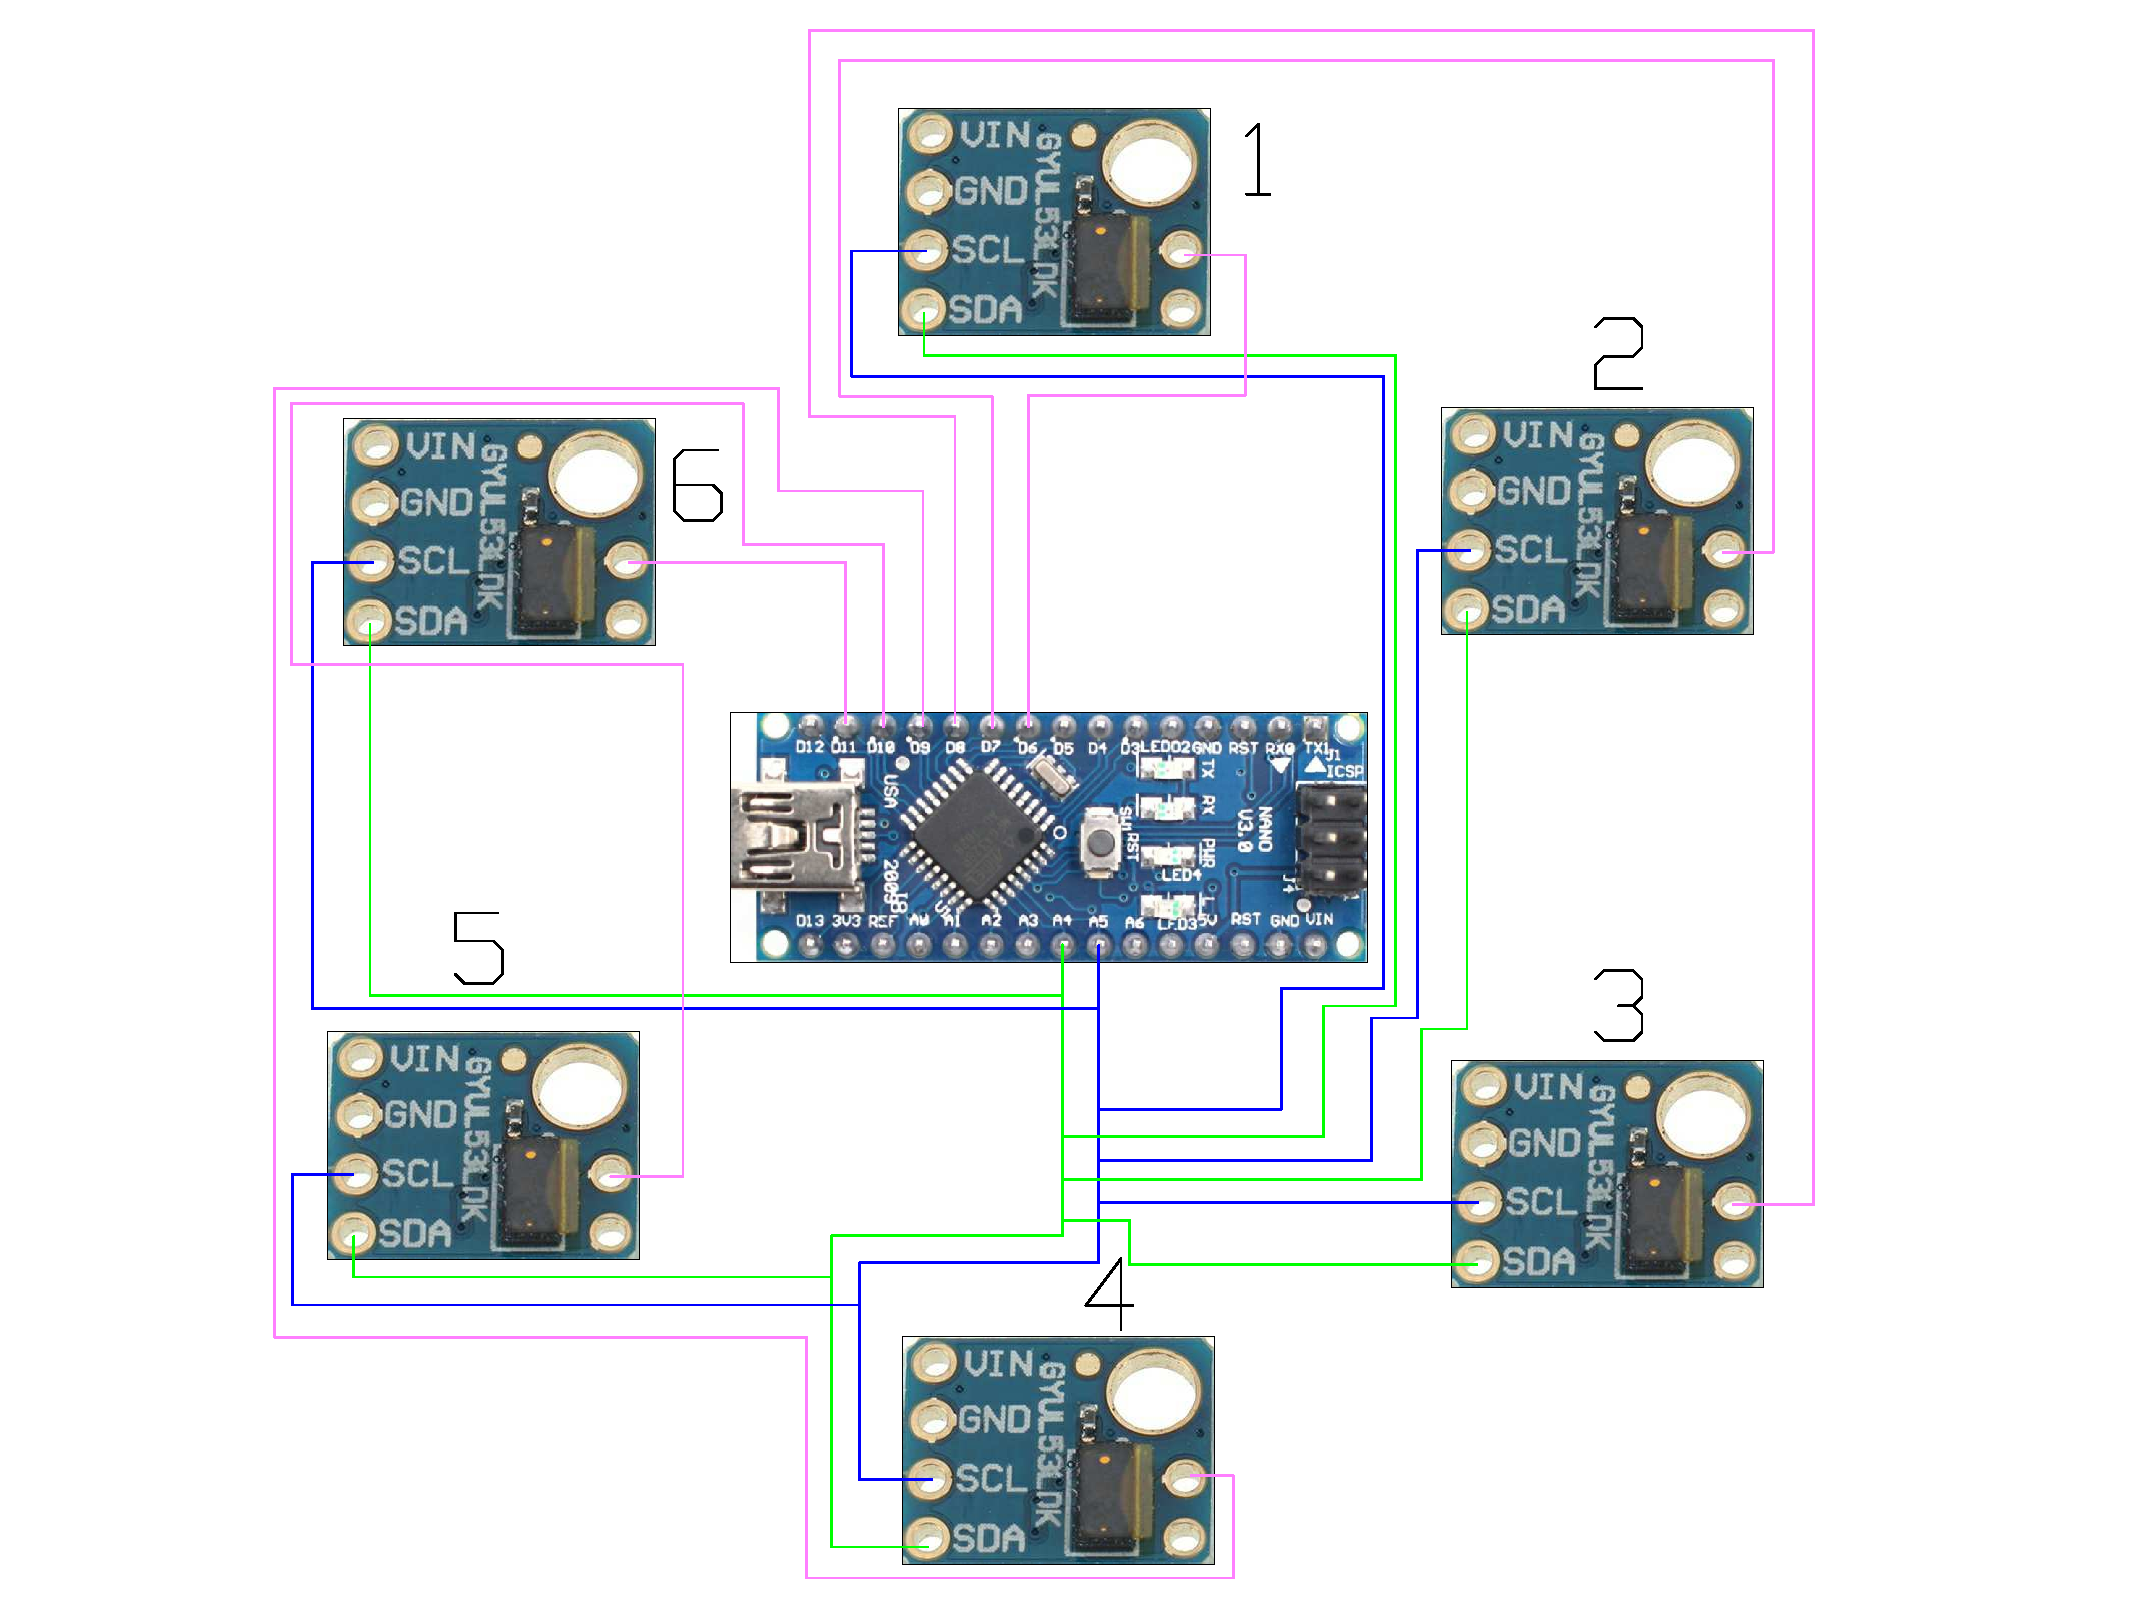
\includegraphics[width=10cm]{pictures/obstacle.pdf}
	\caption{Schéma zapojení Překážkového kontroléru}
\end{figure}

\begin{figure}[h]
	\centering
	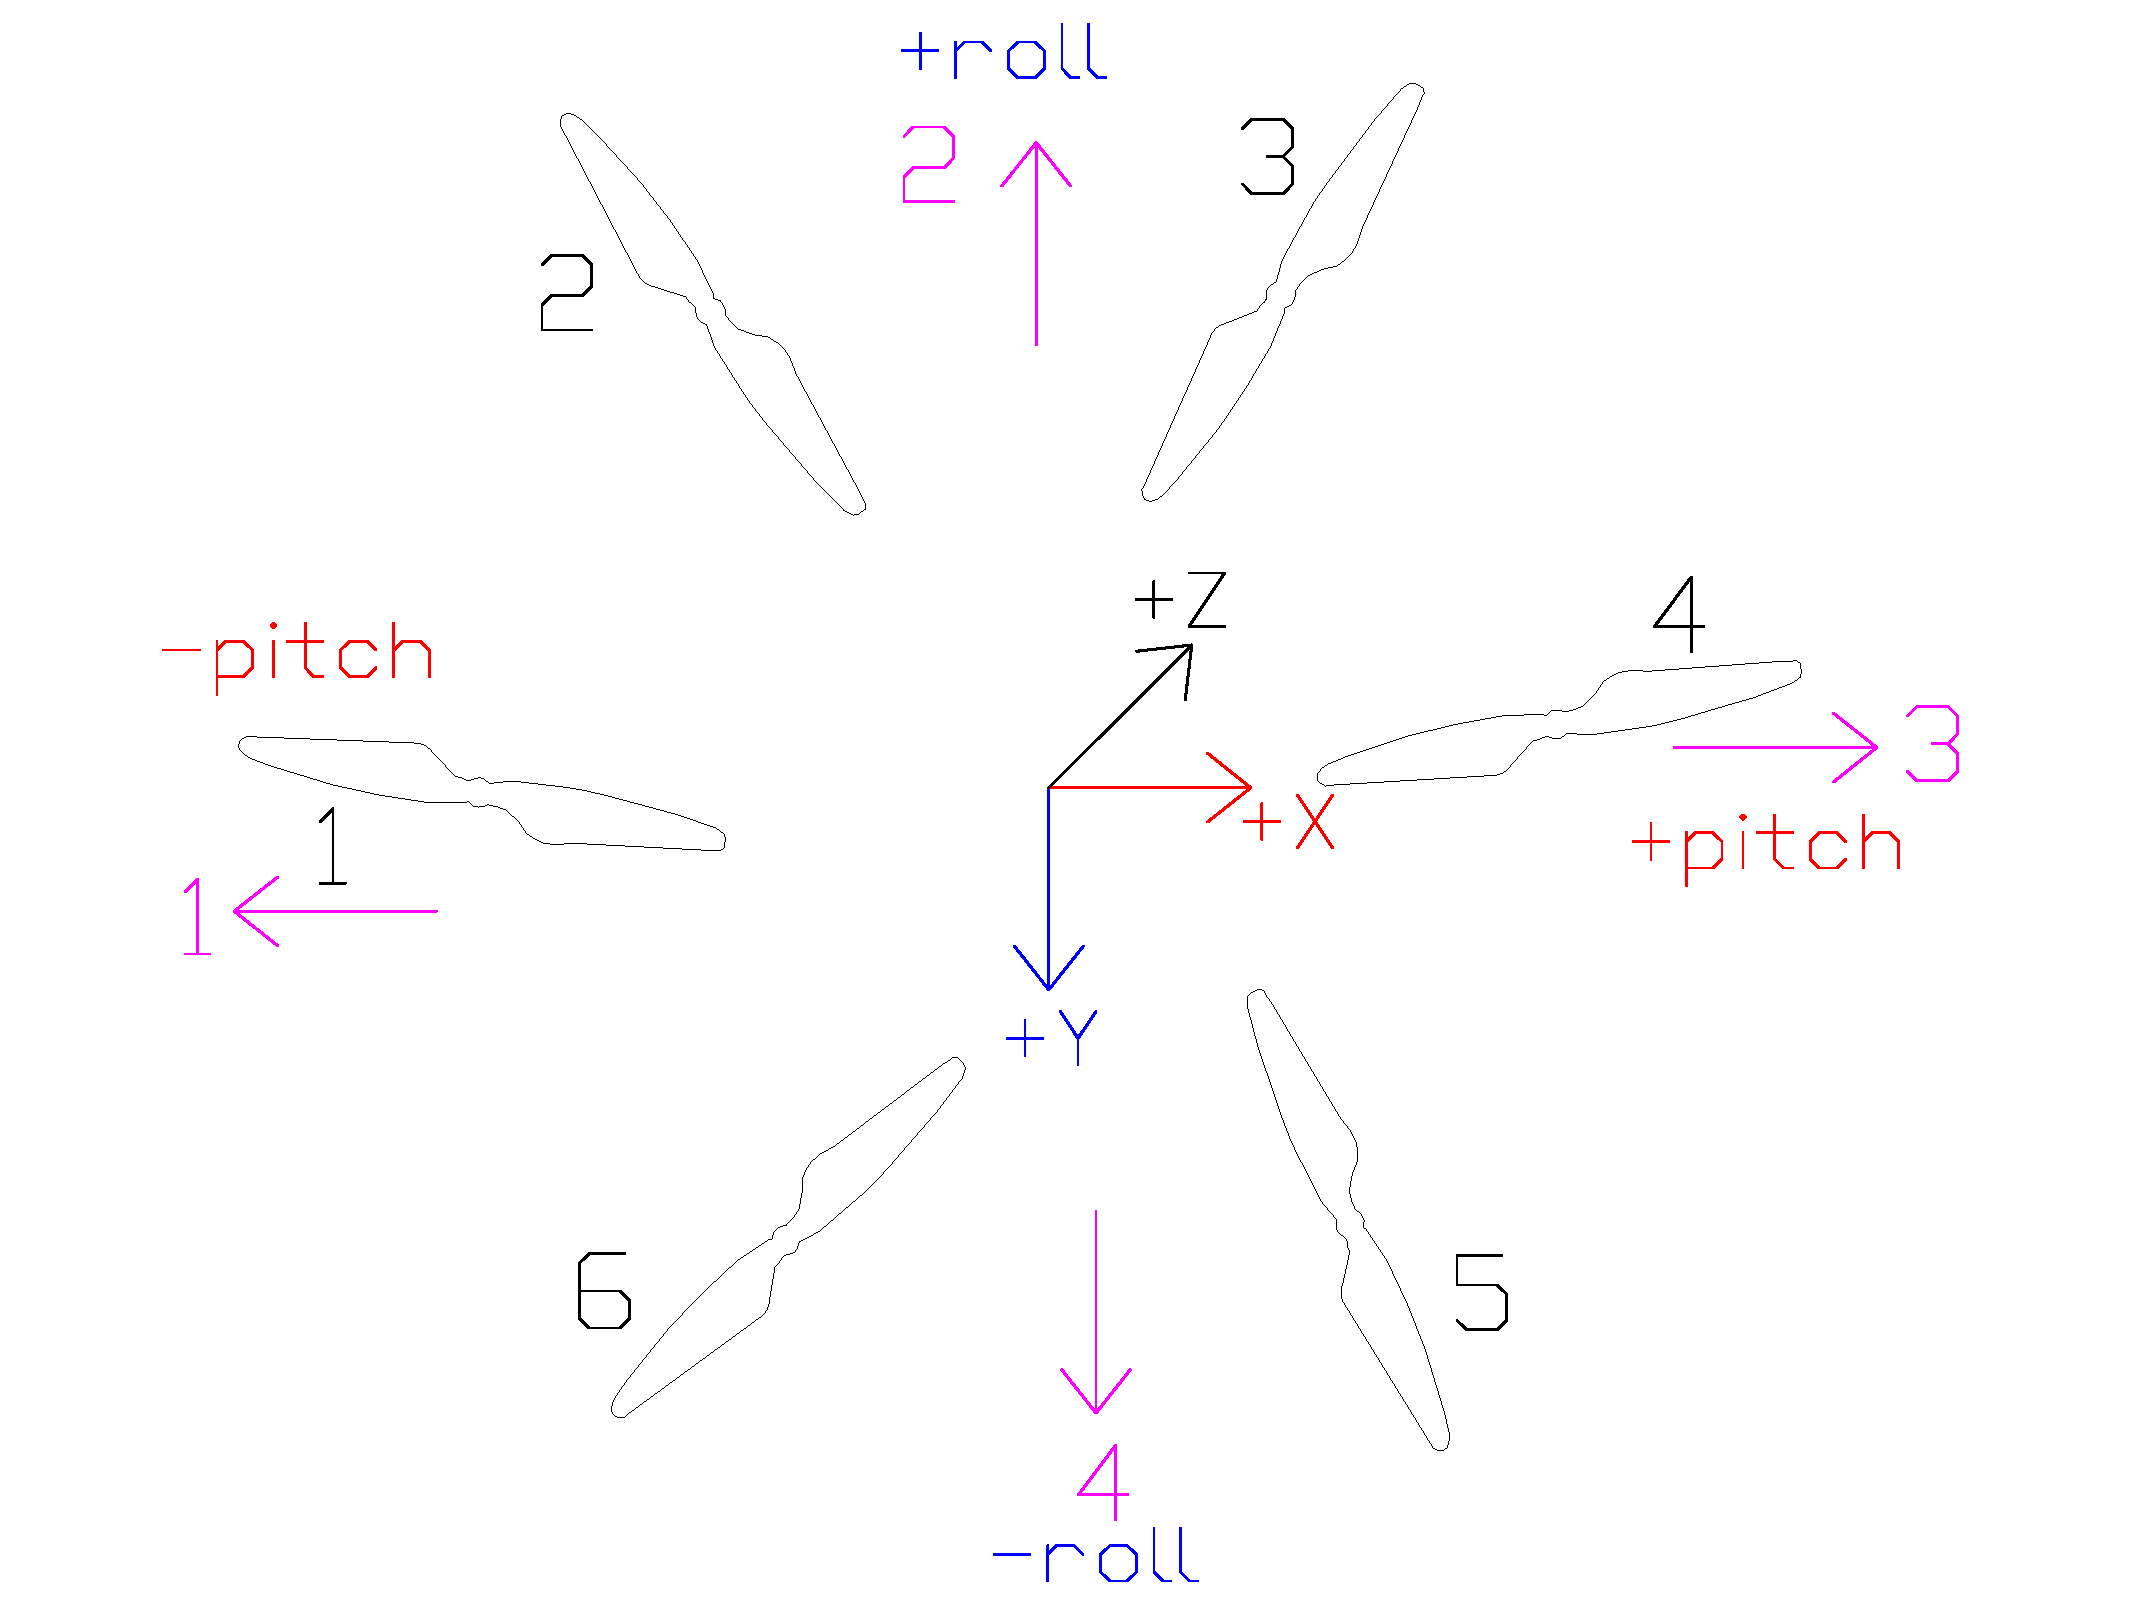
\includegraphics[width=10cm]{pictures/obstacle_teo.pdf}
	\caption{Schéma zpráv překážce}
\end{figure}

\begin{tabbing}
	+/- ~ \= uhel ~~~ \= zprava ~
	\= 34 \kill
	\bfseries +/- \>
	\bfseries Úhel \>
	\bfseries Zpráva \\
	+\> roll \> 2  \\
	-\> roll \> 4  \\
	-\> pitch \> 1  \\
    +\> pitch \> 3  \\
\end{tabbing}

\section{Navigační kontrolér} 
Vstup: Rádio, Bluetooth, Barometr, GNSS, Překážkový kontrolér\\
Výstup: Letový kontrolér\\

Navigační kontrolér složí ke komunikaci s ovládacím zařízením, sběru dat z gnss, barometru a překážkového kontroléru.\\
Používá-li uživatel manuální ovládání, navigační kontrolér pouze ověří zda existuje překážka, pokud existuje, zámezí srážce. Neexistuje-li překážka kontrolér pošle data letovému kontroléru.\\
Při autonomním ovládání kontrolér porovná data z gnss a zadané souřadnice. Pokud souřadnice nejsou totožné, vypočte se směr a vzdálenost z polohy dronu a zadaných souřadnic. Provede se shodnostní transformace ze souřadnicového systému GNSS aparatury do souřadnicového systému dronu. Vstupní data pro PID regulátor budou souřadnicové rozdíly v souřadnicovém systému dronu a výstupní data budou úhly pitch a roll.\\
Při držení určité nadmořské výšky zvovu se použije PID regulátor. Vstupním datem bude nadmořská výška z GNSS aparatury nebo z barometru, výstupem bude výkon motoru, který bude konstatní pro všechny motory.\\
Po zapnutí kontrolér bude čekat na zprávu ze smartphonu. Podle typu příchozích dat kontrolér nastaví autonomní nebo manuální řízení. Při manuální pouze zkontroluje zda existuje překážka a pošle data létovému kontroleru. Při autonomním řízení přečte data z GNSS aparatury, barometru, vypočte transformaci mezi souř. systémem GNSS a dronu. PID regulátory vypočtou úhly pitch, roll a konstantní výkon motoru. Kontrolér zkontroluje zda existuje překážka a nakonec pošle data letovému kontroleru.\\
Bude definována funkce návrat, při které se dron vrátí na startovní místo. Pozice startovního místa bude změřena GNSS aparaturou automaticky před startem dronu.\\
Navigační kontrolér je ve fázi vývoje, zatím nebyl otestován.\\


\begin{figure}[h]
	\centering
	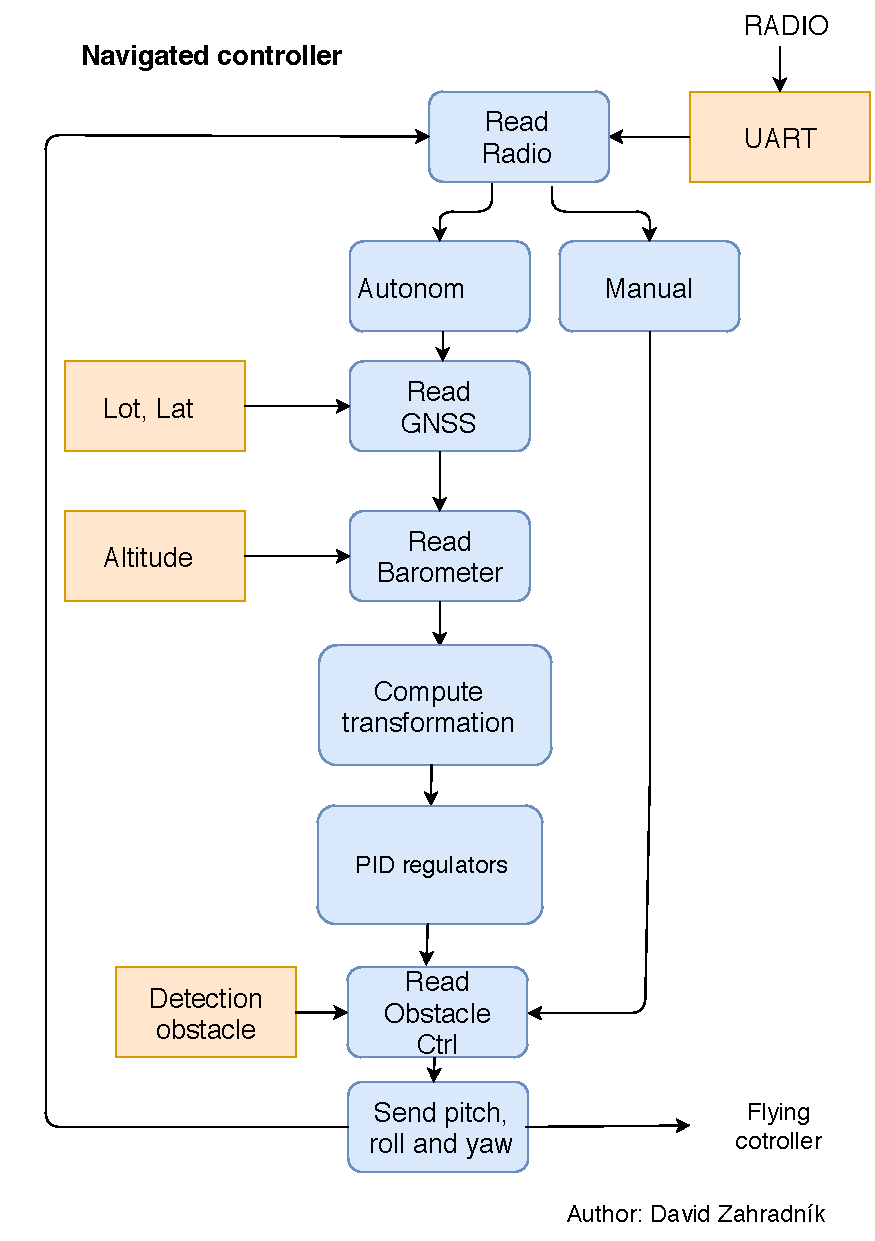
\includegraphics[width=14cm]{pictures/NaviDiagram.pdf}
	\caption{Diagram navigačního kontroléru}
\end{figure}

\section{Finální sestavení}
Z důvodů nízského výpočetního výkonu platfromy Arduino je komplení ovládání sestaveno ze tří platforem Arduino. Letový kontrolér ovládá jednotlivé motory, překážkový kontrolér detekuje případné překážky a navigační kontrolér komunikuje s ovladačem a řídí let.\\
Dron je ovládán smartphonem přes uzlové zařízení. Uzlové zařízení se skládá z bluetooth a radiového modulu. Tok dat probíhá ze smartphonu přes bluetooth do uzlového zařízení a ze zařízení do navigačního kontroléru přes radiový signál.\\
Kamera posílá data smartphonu nezávisle na ovládání dronu. Kamera obsahuje vlastní radiový vysílač, který vysílá data přijímačky připojeného k smartphonu skrze miniUSB. Pro správnou funkci kamery musí mobil podporovat funkci OTG.\\ 

\begin{figure}[h]
	\centering
	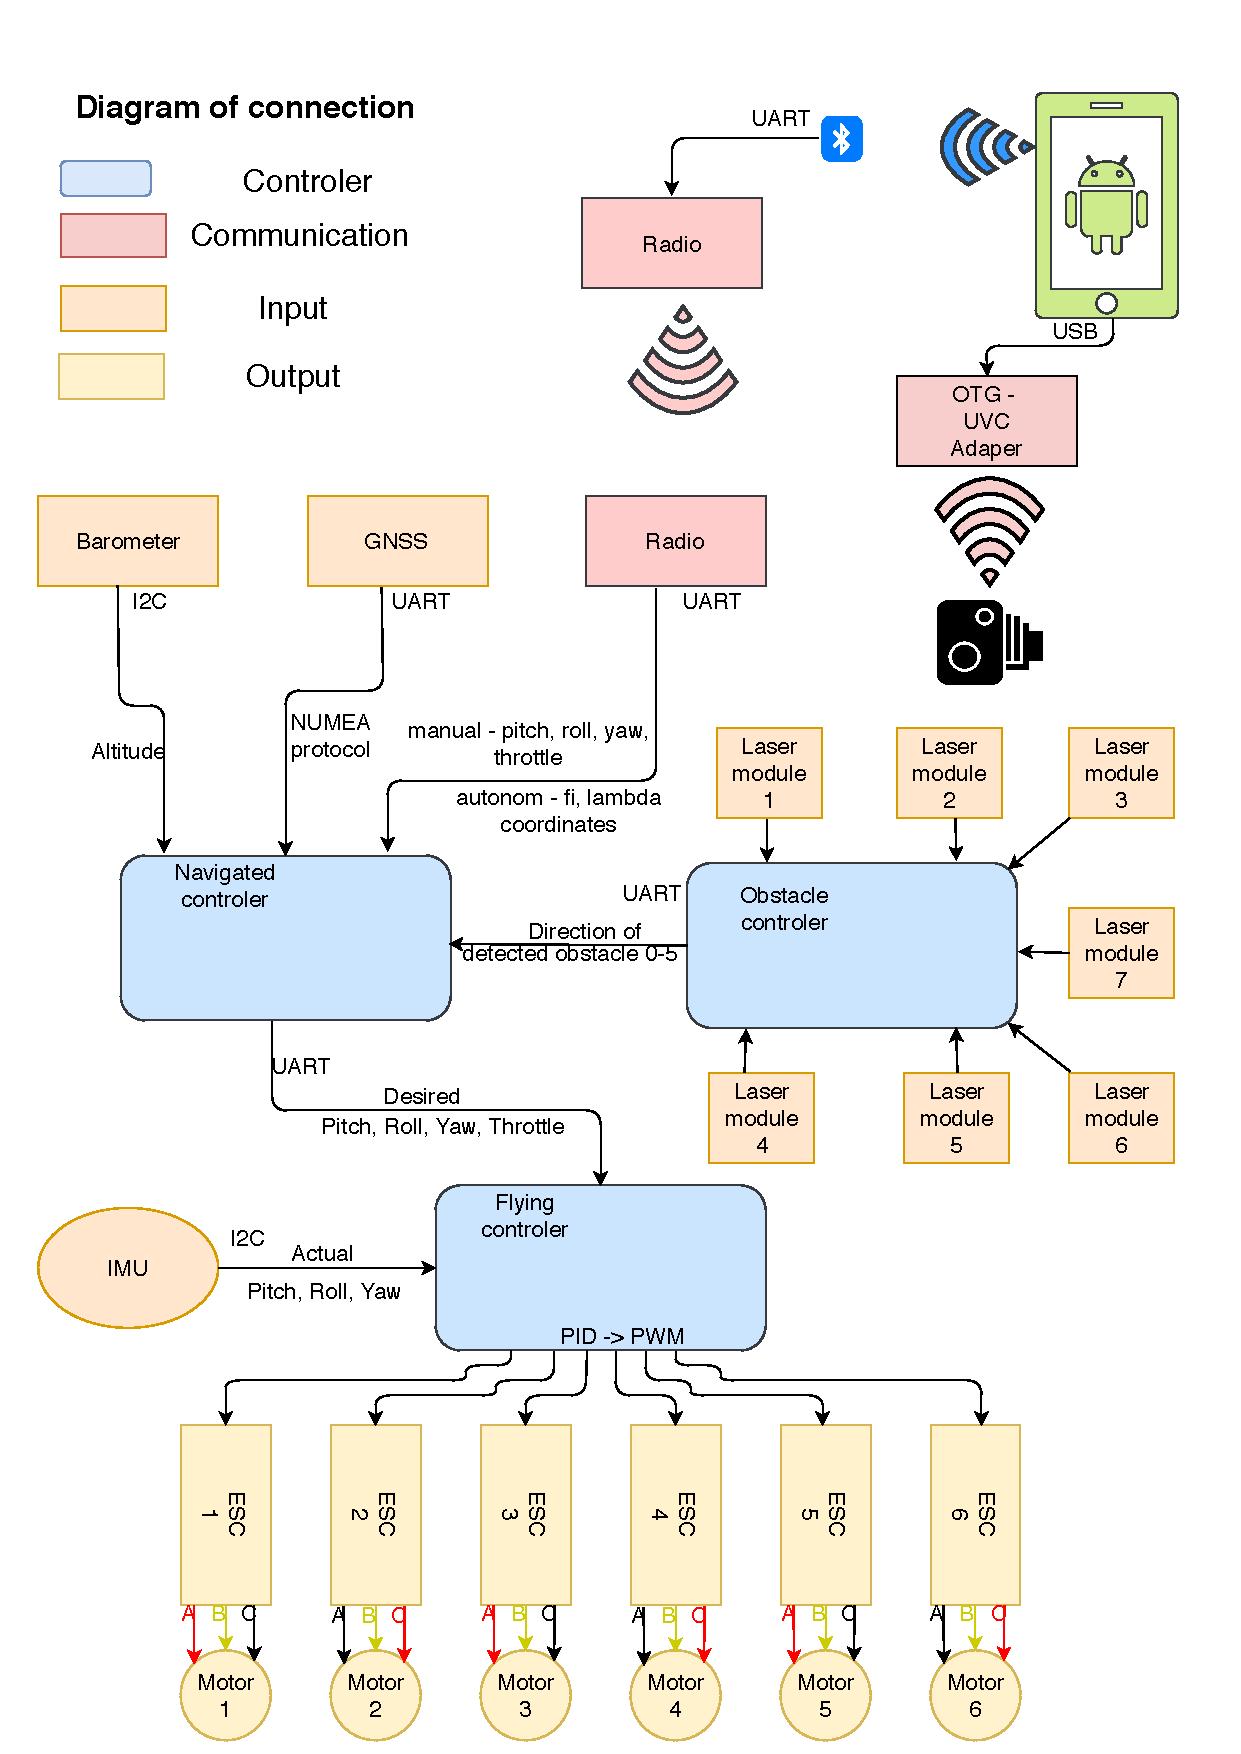
\includegraphics[width=15cm]{pictures/DroneDiagram.pdf}
	\caption{Diagram komponent}
\end{figure}
\begin{figure}[h]
	\centering
	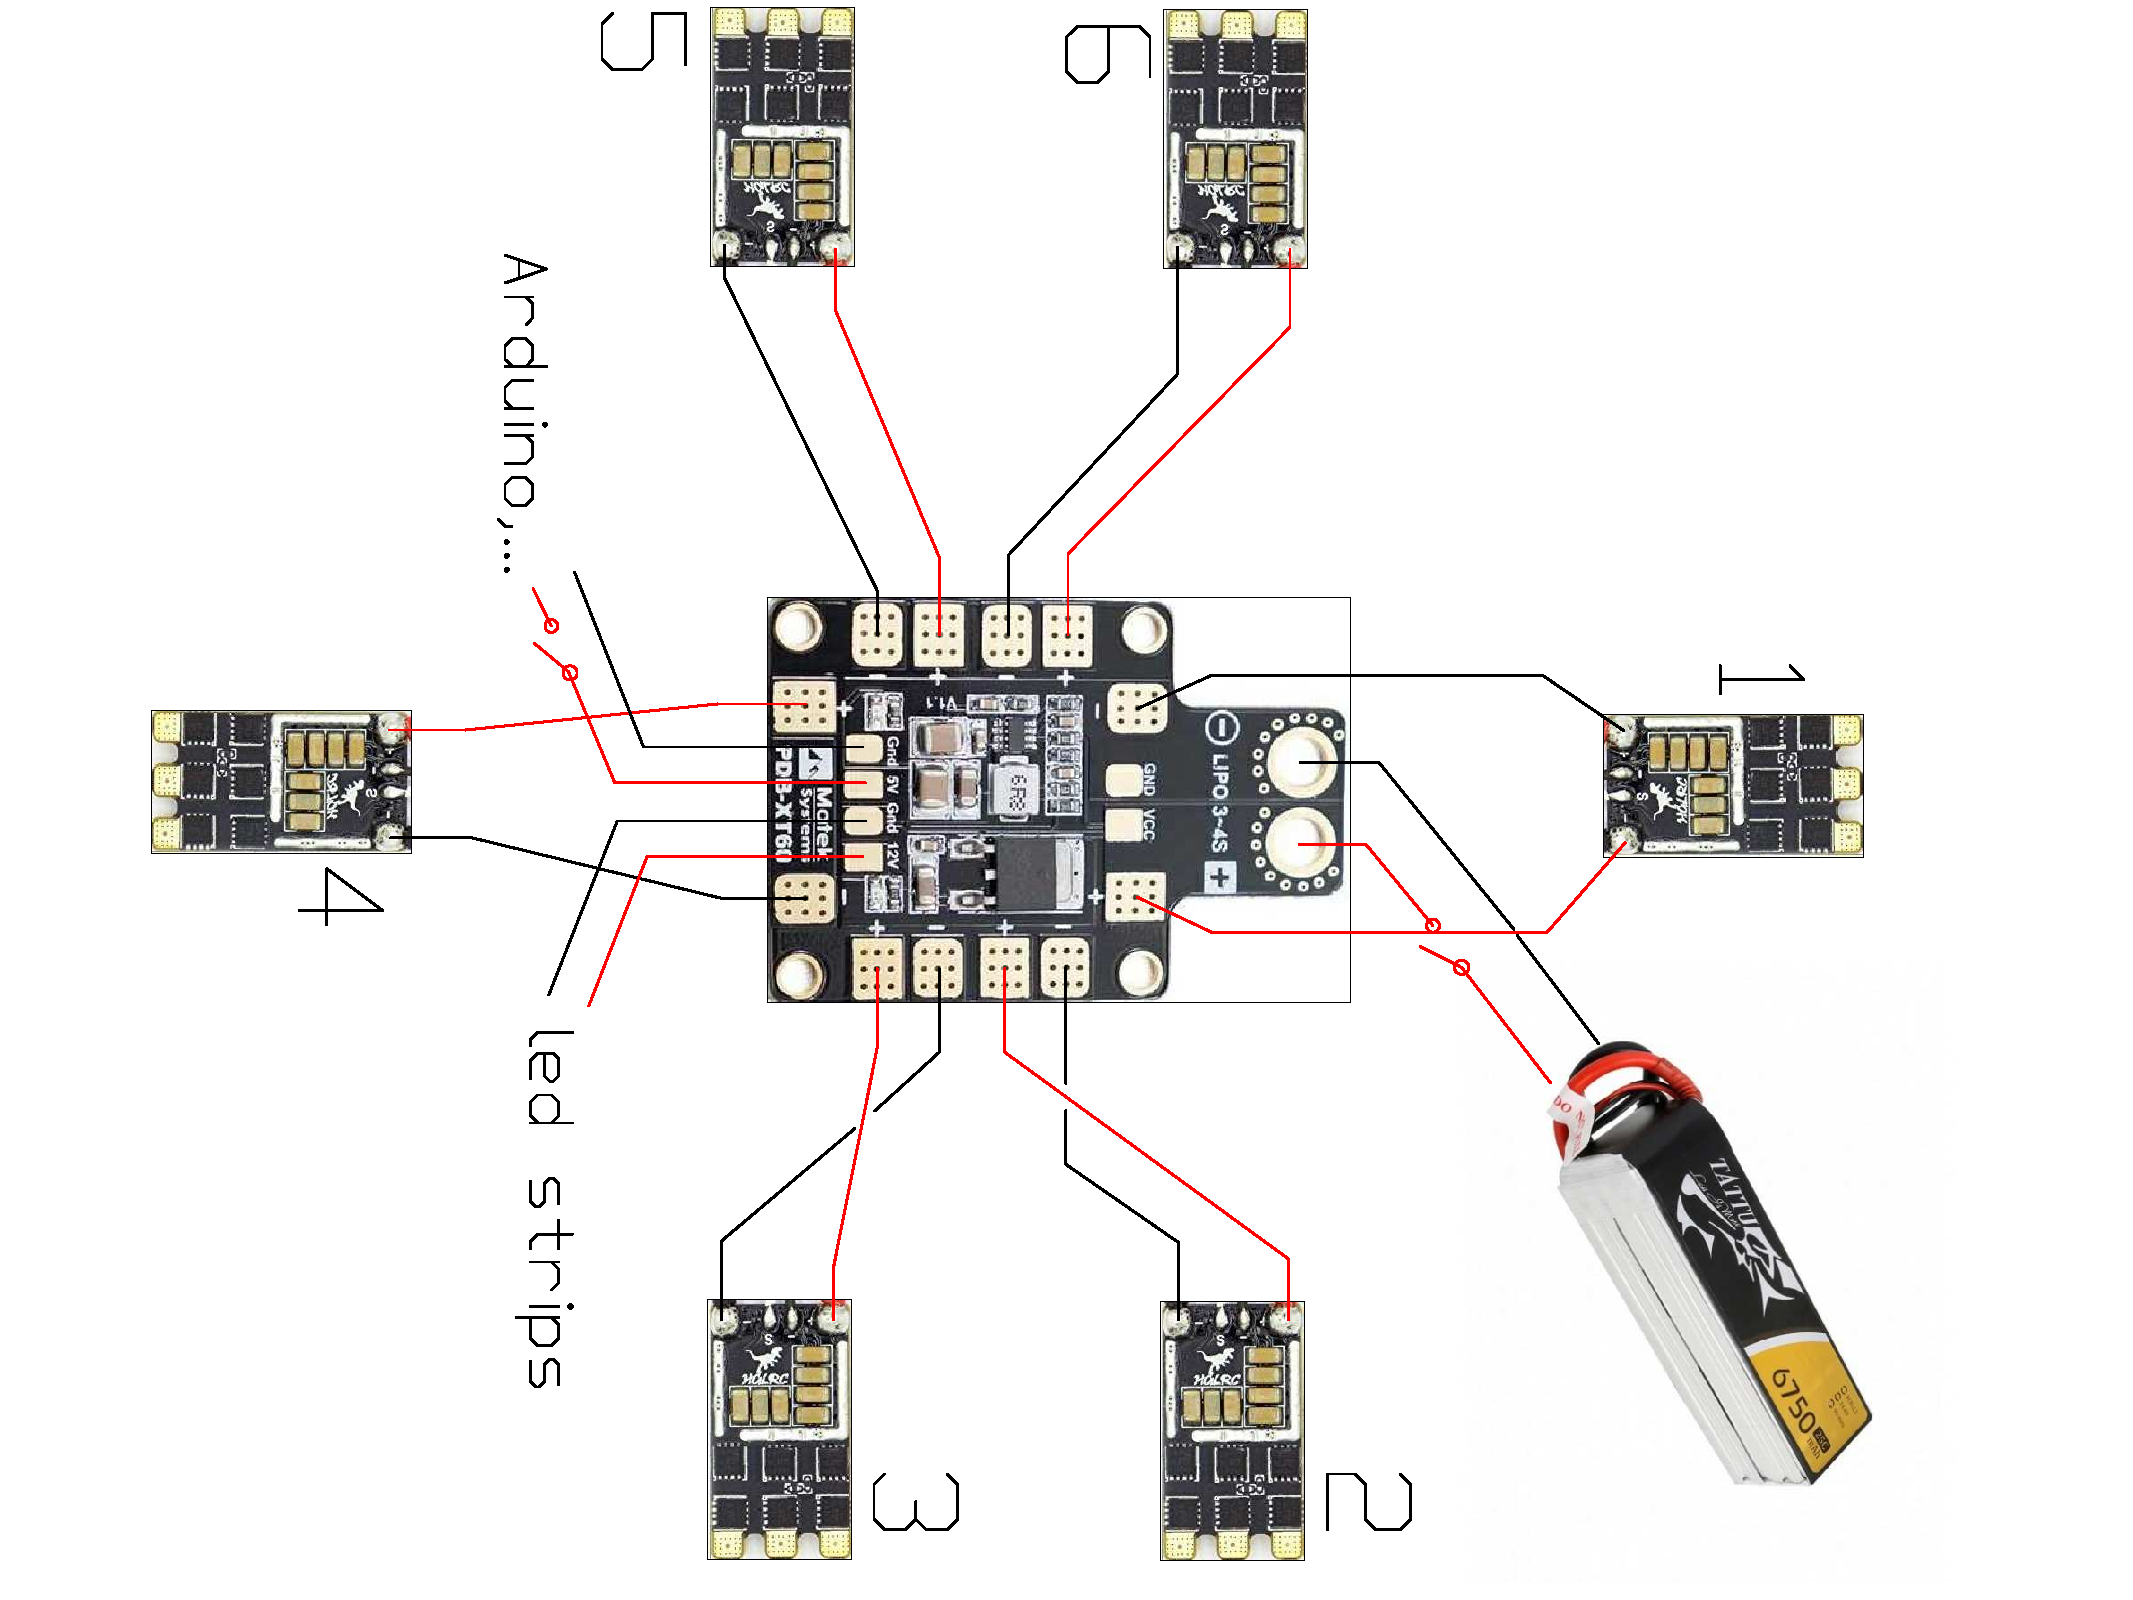
\includegraphics[width=10cm, angle=90]{pictures/pdb_com.pdf}
	\caption{Schéma zapojení napájení motorů}
\end{figure}
\begin{figure}[h]
	\centering
	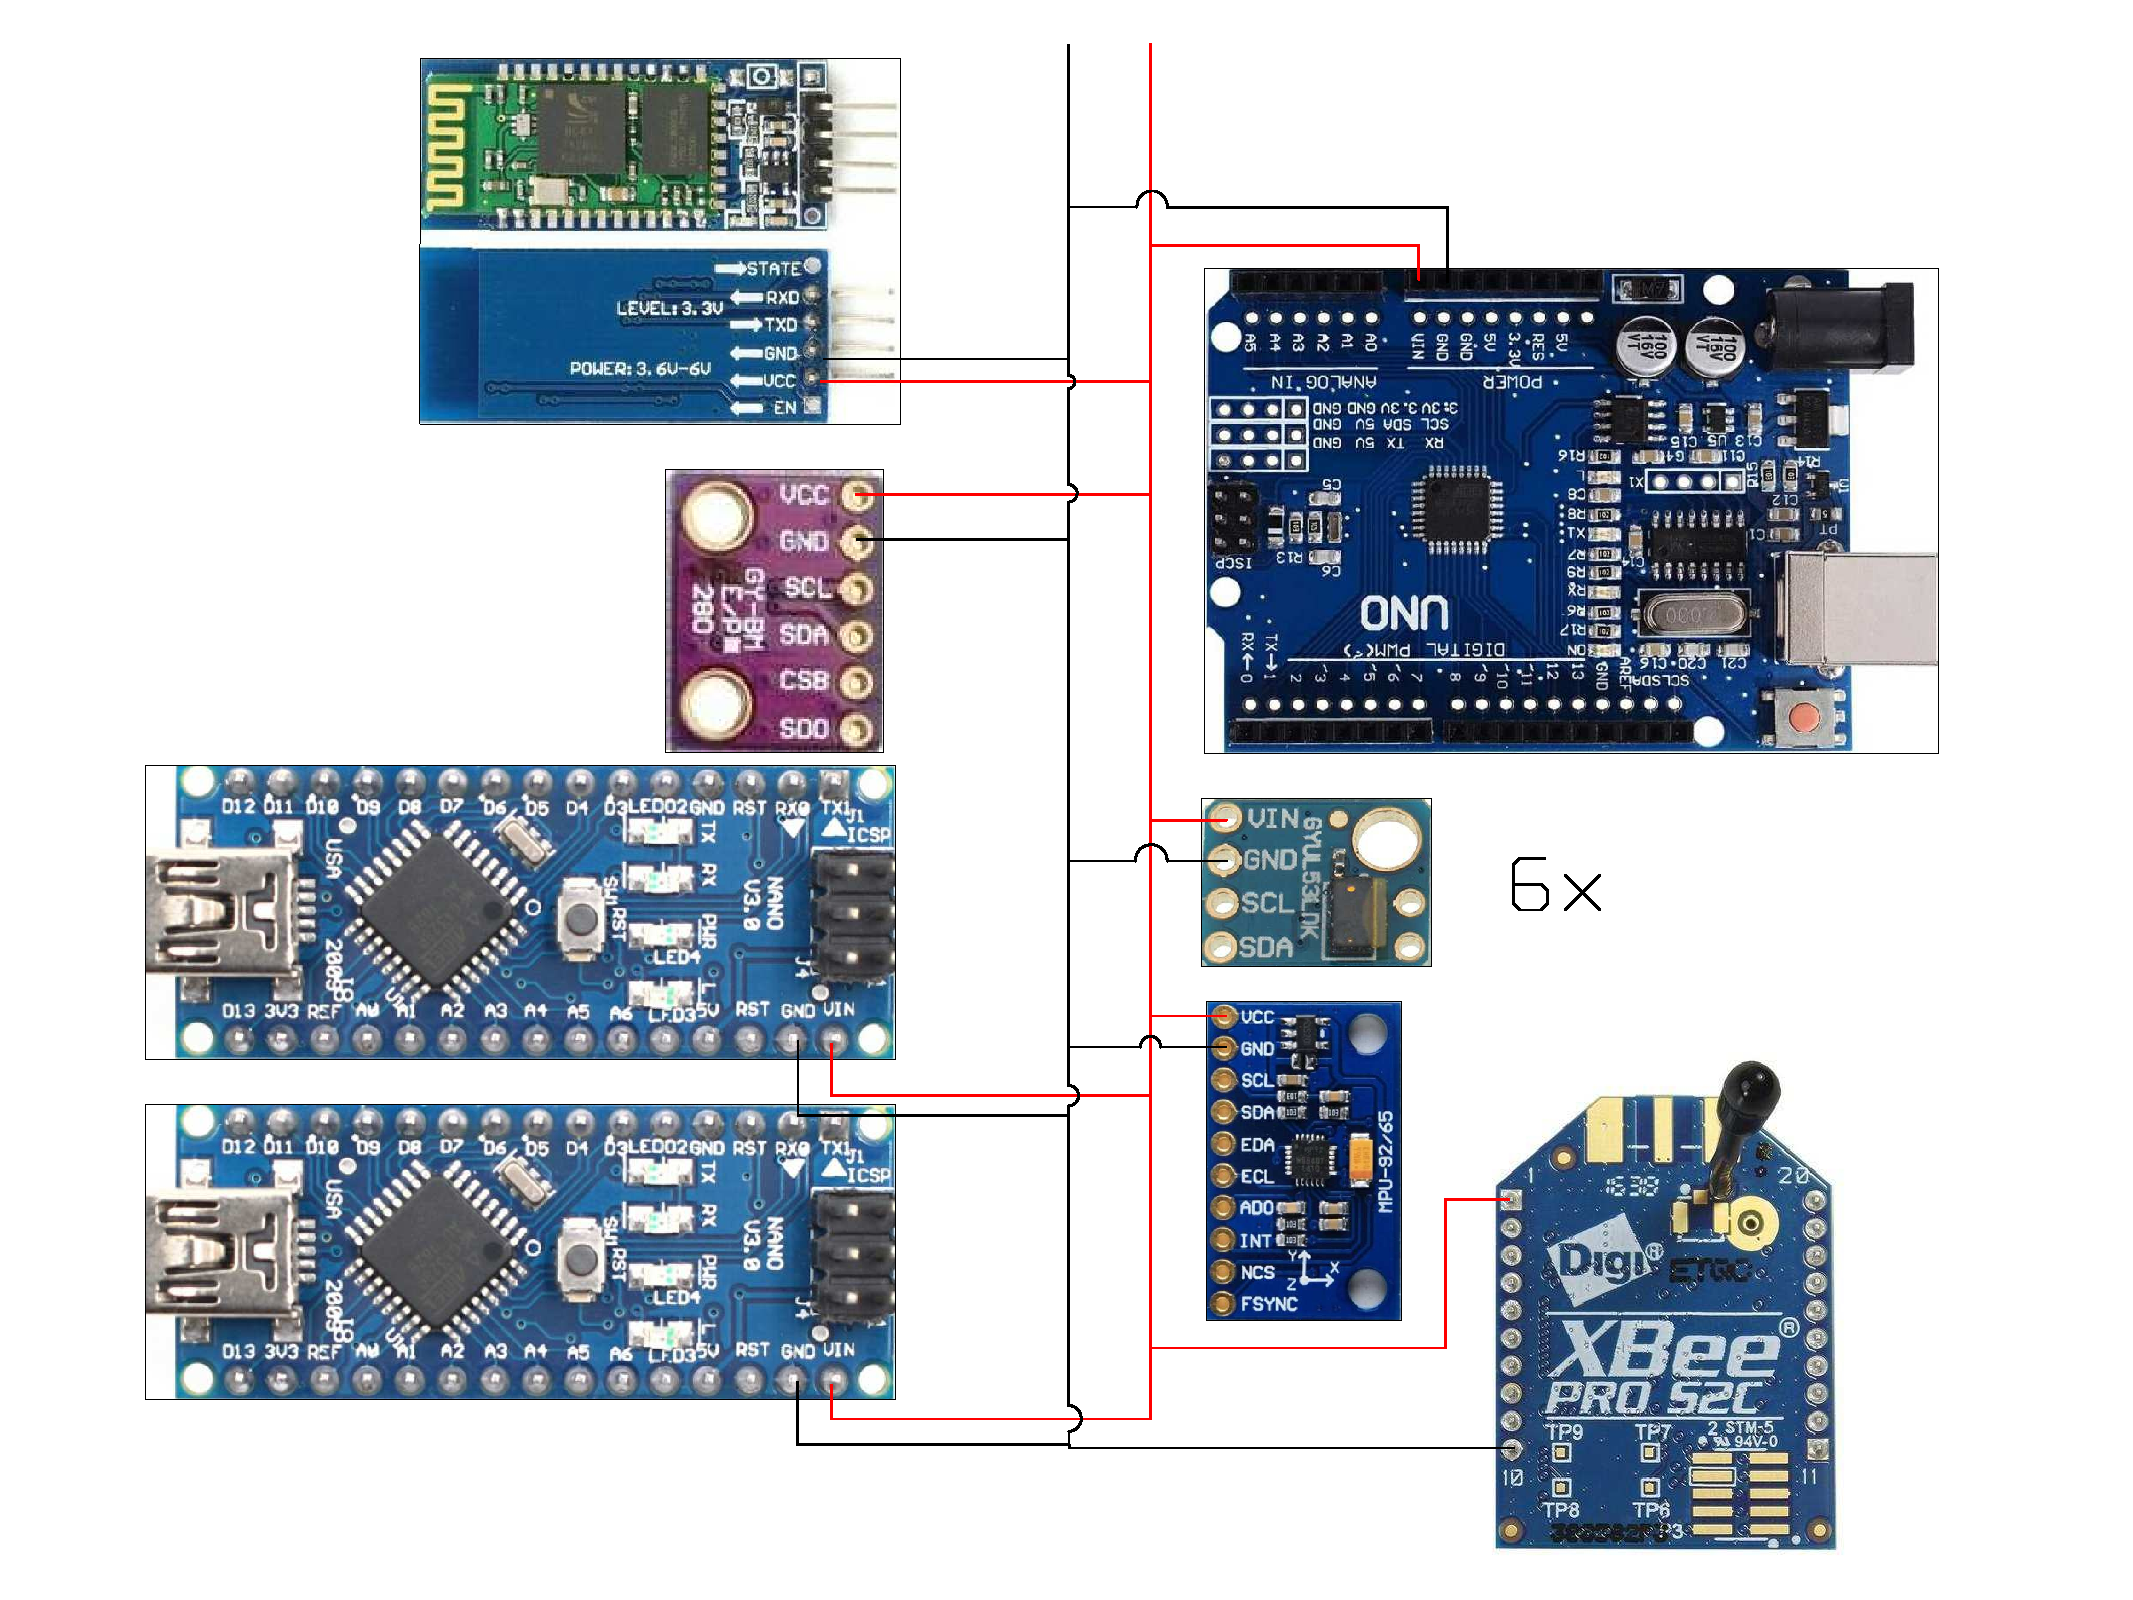
\includegraphics[width=10cm]{pictures/pdb_ardu.pdf}
	\caption{Schéma zapojení napájení Arduina a modulů}
\end{figure}